% -*-coding: iso-latin-1  -*-
% ++++++++++++++++++++++++++++++++++++++++++++++++++++++++++++++++++++++++++++++
% Documento maestros para la elaboraci�n de la tesis  proyectos fin de carrera  y master
%  modificaci�n:	FERNEY BELTRAN
%  Fecha:		    septiembre 2014
% +
%+++++++++++++++++++++++++++++++++++++++++++++++++++++++++++++++++++++++++++++

% Los ficheros necesarios para este documento son:
%
%   Varios/* : 		ficheros con las partes del documento que no
%                   son cap�tulos ni ap�ndices (p�rtada, agradecimientos,
%                   bibliografia etc.) 	
%   Capitulos/*.tex : cap��tulos de la tesis       
%	Apendices/*.tex:  ap�ndices de la tesis       
%	Config/*:			
%			constantes.tex : constantes del documento       
%			config.tex : 	 configuraci�n del documento en general y de  
%							 las plantillas del mismo
%   tmp/:	usado para los  ficheros temporales de compilaci�n
%				
%	se utiliza el entorno de edicion de  eclipse con el  plugin Texlipse
%   para el glosario y los acr�nimos se utiliza el paquete glossaries y
%   para su complilacion se utiliza el script en pearl '\makeglossaries'
%	Para que la compilaci�n se realice en eclipse se debe crear el make
%   glossaries en external tool configuration mas informaci�n en 
%   http://tex.stackexchange.com/questions/45416/using-glossaries-in-texlipse
%.
%	configuraci�n de eclipse :
%	1.)	Incluir en windows ->Preferences -> Texlipse -> Latex Temp File 
%		.acn, .acr, .alg, .glo, .xdy , .ist, .gls, .glg
%	2.) Run -> External Tools -> External Tools config .. program 
%		en location 			selecionar el path de 	/usr/bin/makeglossaries
%       en working Directory 	${project_loc}/tmp
%		en Argument				-q ${project_name} si el .tex es el mismo nombre 
%   3.) Project->Properties->Builders
%		 Selecionar import  y seleccionar la build anteriormente configurado
%   
%   nota: en algunos casos no se crea de forma inmediata el pdf o dvi con los
% acronimos. Para solucionar este inconveniente  se puede generar  el build del
% proyecto  2 o 3 veces seguidas. Otra forma es crear en external tolls config
% un nuevo  build para latex y dvipdf igual que el paso 2 y 3 anterior.  de
% esta forma la configuración de los builders del proyecto podria quedar de la
% siguiente forma:
% 		latex -> makeglossaries -> latex ->latex -> dvipdf 
%
% La segunda opcion es usar el makefile que acompa�a este documento. ejecutarlo
% desde una terminar o configura  eclipse de la siguiente forma.
% 1 Run -> External Tools -> External Tools config .. program 
%		en location 	selecionar el path de make. Donde esta el script  que
%                       ejecuta el makefile, (en linux lo sabe ejecutando 
%                       whereis make) 
% 2 En working Directory ${project_loc} 	
% 3 En Argument          coloque el que m�s le convenga: latex, pdflatex, 
%                        fastlatex, fastpdf 
% 4  En Project ->Properties -> builders -> selecionar el nmbre anteriormente
% creado y, en la pesta�a build options, seleccionar during builds. 
%
% Para el clean, repetir paso 1 y 2 dle proceso anterior, y en arguments
% colocar clean y en la ventana build options, seleccionar unicamente during
% Clean.
% Para hacer el bakups ejecute Makefile zipBackup
% COMENTARIOS 
% Para los comentario o cosas pendientes se recomiendao  usar el comando \TODO,
% definido en el archivo config.tex
% Para los comentarios del Director de tesis usar \commentDir
	
\documentclass[12pt,a4paper, twoside,spanish ]{book}


%% fichero de configuraci�n
% si estamos en debug o release
% en modo debug   se debe comentar el release

% \def\release{1}

\ifx\release\undefined
    % modo debug
    \def\debugmode{1}
    \def\printtodos{1}
    \def\printcoments{1}
    \def\nolayoutconfig{1}
    %\psdraft % no aparecen las imágenes en el documento  impreso
    \def\nogeneratoc{1}
    \def\nogeneraacronimos{1}

\fi



%%%TEXTO

\usepackage{verbatim}		% texto ascii puro tal cual
\usepackage{geometry}		% para la configuración personal de margenes
\usepackage[spanish]{layout}	% depuración de la config de las paginas
				% se incluye el comando \layout en el
				% documento para ver la información de config de pag.

%\usepackage[ansinew]{inputenc}	% windows
\usepackage[T1]{fontenc}		% codificación de las fuentes de  salidas
\usepackage{textcomp}
% \usepackage[latin1]{inputenc}  	% codificación de fuentes
% de entrada \usepackage[utf8]{inputenc}  		% utf8
\usepackage[utf8]{inputenc}
\usepackage[round]{natbib}	% soporte para bibliografía
				% \citep{ref} entre paréntesis
				% \citet{ref} cita normal
				% \citeyear{ref} para la fecha
				% \citeauthor{ref}
				% http://merkel.zoneo.net/Latex/natbib.php


% \usepackage[spanish]{babel}
\usepackage[spanish,activeacute]{babel}	% Soporte para castellano
\fontfamily{garamond}

\usepackage{xcolor}

%% PÁRRAFOS

\usepackage{multicol}		% utilización de multicolumna
\setlength{\parskip}{0.2ex} 	% separación entre párrafos se aumenta
\newcommand{\linespacing}[1]{\renewcommand{\baselinestretch}{#1}\normalsize}

%% TÍTULOS

\usepackage{titlesec} 	% Cambia el formato de los  títulos
			% importante para la definición de encabezados
			% \chaptertitlename, -> \chaptername ("Capítulo")
			% o  a \apendixname ("Apéndice")



% DIRECCIONES WEB

\usepackage{url}		% soporte para incluir dirección. web
				% \url{http://...}
\usepackage{ifpdf}		% para compilaciones con pdflatex
				% en lugar de latex, se define el ifpdf
\ifpdf				% Color y borde de los enlaces
  \RequirePackage[pdfborder=0,colorlinks,hyperindex,pdfpagelabels]{hyperref}
  \def\pdfBorderAttrs{/Border [0 0 0] }
\else
  \usepackage{hyperref}
\fi
\hypersetup{colorlinks=false}


%%  IMAGENES

\usepackage{subfig}		
\usepackage{epsfig}		% imágenes eps
\usepackage{epsf}              % Ciertas manipulaciones a EPSs
% \usepackage[final]{graphicx}
% \usepackage[draft,dvips]{graphicx}
% \usepackage[pdftex]{graphicx}		% para imágenes  JPG PNG PDF

\usepackage{tikz}
\usetikzlibrary{mindmap, trees,backgrounds}

%% TABLAS

\usepackage{tabularx}		% hacer tablas con párrafos
\usepackage{longtable}		% tablas de  varias hojas
\renewcommand{\arraystretch}{1.2}	%(or 1.3) %más espacio entre las lineas de la tabla
\usepackage{colortbl}			% color en la tablas
\usepackage{color}
\usepackage{booktabs} 			% Para poner las tablas elegantes



% MATEMÁTICAS

\usepackage{calc}      % ayuda con cálculos  básicos dentro de latex
\usepackage{amsmath}   % From the American Mathematical Society
\usepackage{amssymb}


%% ACRONIMOS

%% inclusión del paquete glossaries, para  tener los acrónimos
%	xindy 	indica que el motor de  búsqueda es xindy, se necesita del  la instalación de xindy
%	acronym, indica que se genera lista de acrónimos
%	nomumberlist	para  que no incluya la pagina donde aparece el acrónimo
%	sanitize=none evita lso problemas con los acentos  en algunos comandos
%	\ac muestra el acrónimo en su forma  completa la primera vez  que se llama y
%       la forma corta las siguientes 	
%   \ac1 muestra la  forma larga del acrónimo
%	\acs muestra la forma corta y \acf la forma completa
% el fichero fuente esta en bd_acronimos

\usepackage[xindy={language=spanish-traditional},
acronym, nonumberlist,translate=false,toc,
shortcuts,hyperfirst=false,sanitize=none]{glossaries}



%%  OTROS

% Redefinición al español los nombres de las  tablas  e índices, ya que
% el paquete babel  los pone con el nombre de cuadros
\addto\captionsspanish{%
  \def\tablename{Tabla}%
  \def\listtablename{\'Indice de tablas}%
  \def\listfigurename{\'Indice de figuras}
  \def\contentsname{\'Indice general}%
  \def\chaptername{Cap\'itulo}%
  \def\listacronymname{Acrónimos y abreviaturas}%
  \renewcommand*{\acronymname}{Acrónimos y abreviaturas}
  \renewcommand*{\glossaryname}{Glosario}
}


%% GENERACIÓN DE NUEVOS COMANDOS  PARA SIMPLIFICAR LA ESCRITURA

% insertar una figura con el fin de evitar la inclusion de la carperta
% en donde estan las imagenes

%\newcommand{\imagen}[2]{%
%  \includegraphics[#2]{image/#1}%
% }

% insertar figuras directamente desde el texto, se debe indicar 4
% argumentos 1 el nombre del fichero, 2 width=Xcm,height=Ycm,angle=Z,
% 3 la etiqueta de la figura y 4 el titulo de la misma
\newcommand{\figura}[4]{%
  \begin{figure}[t]%
    \begin{center}%
      \imagen{#1}{#2}%
      \caption{#4} \label{#3}%
    \end{center}%
  \end{figure}%
}


% Configuración del resumen de cada capitulo
\newenvironment{resumen}{%
\begin{quotation}\noindent\begin{small}\textbf{\textsc{Resumen:}}%
}%
{%
\end{small}\end{quotation}%
\bigskip%
}

% configuración de comentarios y cosas por hacer

% TODO
\newcommand{\TODO}[1]{{\color{orange} TODO: #1}}
% comentarios Director
\newcommand{\commentDir}[1]{{\color{red} Comentarios Director: #1}}


%%% FIN CONFIG


%% Config de cabeceras de capitulos  y secciones especiales
\usepackage{fancyhdr}			% Cambia los parámetros de la cabecera
\pagestyle{fancy}			    % elegir este estilo de cpps
\addtolength{\headheight}{2pt}	% se evitan warnings por el tamaño de la cabecera


\newcommand{\restauraCabecera}{
  \fancyhead[LO]{\rightmark}
  \fancyhead[RE]{\leftmark}
}


\renewcommand{\headrulewidth}{0.5pt}             % Cabecera: subraya la cabecera (fijar en "0pt" si no se desea).
\renewcommand{\footrulewidth}{0pt}               % Pié: subraya el pie de página (fijar en "0pt" si no se desea).
\renewcommand{\chaptermark}[1]{%
   \markboth{\textsc{\chaptertitlename\ \thechapter.}\ #1}{}%
}
\renewcommand{\sectionmark}[1]{\markright{\thesection.\ #1}}
\fancyhf{}
\restauraCabecera
\fancyhead[RO,LE]{\thepage}
\fancyhead[LE,RO]{\textbf{\thepage}}           % Cabecera: número de página en negrita.

% para los capítulos que  no tiene numeración  ni secciones  se debe cambiar
\newcommand{\cabeceraEspecial}[1]{
  \fancyhead[LO]{\textsc{#1}}
  \fancyhead[RE]{\textsc{#1}}
}

\newcommand{\Resumen}{Resumen\markright{Resumen}}
%\newcommand{\TocResumen}{\addcontentsline{toc}{section}{Resumen}}


\newcommand{\Conclusiones}{Conclusiones\markright{Conclusiones\ldots}}
%\newcommand{\TocConclusiones}{\addcontentsline{toc}{section}{Conclusiones}}


% Definición del estilo en la  página de inicio de capítulo: Número de
% la página abajo a la derecha, y sin línea en la zona superior.
\fancypagestyle{plain}{%
  \fancyhf{}
  \fancyfoot[R]{\thepage}
  \renewcommand{\headrulewidth}{0pt}
  \renewcommand{\footrulewidth}{0pt}
}

%% Prevenir que al cambiar de capitulo la pagina en blanco no tenga cabecera
\makeatletter
\def\cleardoublepage{\clearpage\if@twoside \ifodd\c@page\else
  \hbox{}
  \thispagestyle{empty}
  \newpage
  \if@twocolumn\hbox{}\newpage\fi\fi\fi}
\makeatother


% Saber que se esta en modo Debug,

\ifx\release\undefined
  \fancyfoot[LE,RO]{\vspace*{1cm}\small \sc Draft   -- \today}
\fi


% Fichero con las macros para crear la bibliografia
%\include{config/config_bib}

 % fichero de las constantes a usar en el documento
% -*-%---------------------------------------------------------------------
%
%                          constantes.tex
%
\def\tipoDoc{ Tesis } % tesis Articulo, Documento

\ifx\release\undefined
  \def\nombreDoc{[DRAFT] Tesis Doctoral }
\else
  \def\nombreDoc{Tesis Doctoral }
\fi

% \def\tituloDoc{ Relating the Spectrum of Cardiac Signals to the Spatiotemporal Dynamics of Cardiac Source }
\def\tituloDoc{ Relación entre el espectro de señales cardiacas y la dinámica
espacio temporal de las fuentes cardiacas}
\def\autorDoc{Ferney Alberto Beltrán Molina }
\def\directorDocA{Jesús Requena Carrión }
\def\directorDocB{Felipe Alonso Atienza }
\def\universidad{Universidad Rey Juan Carlos }

\ifx\nogeneraacronimos\undefine
	\makeglossaries
	% -*-coding: iso-latin-1  -*-

%
% Fichero con acr�nimos para su uso con Glossaries
%
% elaborado por ferney alberto beltr�n
% fecha de creaci�n	 2 de abril de 2013

% La entrada es:
% \newacronym{hlabeli}{habbrvi}{hfulli}

\newacronym{DF}{DF}{Frecuencia Dominante}
\newacronym{AF}{AF}{Fibrilaci�n Auricular}
\newacronym{VF}{VF}{Fibrilaci�n Ventricular}
\newacronym{LF}{LF}{Lead Field}
\newacronym{EGM}{EGM}{Electrocardiograma}

\newacronym{IEEE}{IEEE}{Institute of Electrical and Electronic Engineers}
\newacronym{FABM}{FABM}{FERNEY ALBERTO BELTRAN MOLINA}

\fi
%
% "Metadatos" para el PDF
%

\pdfinfo{
   /Author (\autorDoc)
   /Title  (\tituloDoc)
   /CreationDate (\today)
   /Subject (PDFLaTeX)
   /Keywords (PDF;LaTeX)

}

%\usepackage{fancyhdr}			% Cambia los parámetros de la cabecera
\pagestyle{fancy}			    % elegir este estilo de cpps
\addtolength{\headheight}{2pt}	% se evitan warnings por el tamaño de la cabecera


\newcommand{\restauraCabecera}{
  \fancyhead[LO]{\rightmark}
  \fancyhead[RE]{\leftmark}
}


\renewcommand{\headrulewidth}{0.5pt}             % Cabecera: subraya la cabecera (fijar en "0pt" si no se desea).
\renewcommand{\footrulewidth}{0pt}               % Pié: subraya el pie de página (fijar en "0pt" si no se desea).
\renewcommand{\chaptermark}[1]{%
   \markboth{\textsc{\chaptertitlename\ \thechapter.}\ #1}{}%
}
\renewcommand{\sectionmark}[1]{\markright{\thesection.\ #1}}
\fancyhf{}
\restauraCabecera
\fancyhead[RO,LE]{\thepage}
\fancyhead[LE,RO]{\textbf{\thepage}}           % Cabecera: número de página en negrita.

% para los capítulos que  no tiene numeración  ni secciones  se debe cambiar
\newcommand{\cabeceraEspecial}[1]{
  \fancyhead[LO]{\textsc{#1}}
  \fancyhead[RE]{\textsc{#1}}
}

\newcommand{\Resumen}{Resumen\markright{Resumen}}
%\newcommand{\TocResumen}{\addcontentsline{toc}{section}{Resumen}}


\newcommand{\Conclusiones}{Conclusiones\markright{Conclusiones\ldots}}
%\newcommand{\TocConclusiones}{\addcontentsline{toc}{section}{Conclusiones}}


% Definición del estilo en la  página de inicio de capítulo: Número de
% la página abajo a la derecha, y sin línea en la zona superior.
\fancypagestyle{plain}{%
  \fancyhf{}
  \fancyfoot[R]{\thepage}
  \renewcommand{\headrulewidth}{0pt}
  \renewcommand{\footrulewidth}{0pt}
}

%% Prevenir que al cambiar de capitulo la pagina en blanco no tenga cabecera
\makeatletter
\def\cleardoublepage{\clearpage\if@twoside \ifodd\c@page\else
  \hbox{}
  \thispagestyle{empty}
  \newpage
  \if@twocolumn\hbox{}\newpage\fi\fi\fi}
\makeatother


% Saber que se esta en modo Debug,

\ifx\release\undefined
  \fancyfoot[LE,RO]{\vspace*{1cm}\small \sc Draft   -- \today}
\fi


%%%%%%%%%%%%%%%%%%%%%%%%%%%%%%%%%%%%%%%%%%%%%%%%%
%-----------------document begins here ---------%
%%%%%%%%%%%%%%%%%%%%%%%%%%%%%%%%%%%%%%%%%%%%%%%%%

\begin{document}


\ifx\release\undefined
  \layout		% para ver la configuraci�n de las pagimas
\fi

% -*-coding: iso-latin-1  -*-

\begin{center}

\thispagestyle{empty} %\vspace{0cm}
\begin{figure}[h]
\centering
	
\includegraphics[width=1.3cm]{images/logo_URJC.eps} \label{figure:HS2ant}
	\vspace{-0.5cm}
\end{figure}

\linespacing{1.5}


{\large \universidad} %\vspace{1cm}




 %\rule{.9\textwidth}{0.5pt}

\vfill {\LARGE\bf \nombreDoc }\vspace{0.5cm}

{\Large\bf \textsc \tituloDoc }

% cjbc
%\linespacing{1.2} \vspace{1.5cm}
\vspace{2cm}

{\large Autor:}

{\large\bf \autorDoc}\vspace{1cm}


Directores:

{\large\bf Dr. D. \directorDocA}
\\ {\large\bf Dr. D. \directorDocB}


\vspace{1cm}


\vspace*{1cm} {TEOR�A DE LA SE�AL Y COMUNICACIONES Y SISTEMAS TELEM�TICOS Y COMPUTACI�N}\vspace{1cm}

\large{Fuenlabrada, Diciembre de 2015}
\end{center}
\vspace{2cm}
\clearpage


\frontmatter % estilo que debe tener el documento (p�gina de t�tulo, tabla de
% contenidos, pr�logos),
% N�meros romanos



\chapter{Resumen}
\cabeceraEspecial{Resumen}
inicio del resumen




\endinput
 


\chapter{Abstract}
\cabeceraEspecial{abstract}
In this Doctoral Dissertation  \ldots\ldots




\endinput

%%% -*-coding: iso-latin-1  -*-

\chapter{Dedicatoria}


\endinput
%%% -*-coding: iso-latin-1  -*-


\chapter{Agradecimientos}


\endinput

%% Tablas de Contenidos 
\ifx\nogeneratoc\undefine
  % -*-coding: iso-latin-1  -*-
%config_toc

\setcounter{tocdepth}{2} %  % nivel de subsection en la tabla 
\setcounter{secnumdepth}{3} % nivel de numeraci�n en el documento

 
% Tabla de contenidos.
% \cabeceraEspecial{\'Indice general}

\tableofcontents
\pdfbookmark{Tabla de contenidos}{tabla de contenidos}
 
\newpage 
% �ndice de figuras

\listoffigures
\pdfbookmark[1]{�ndice de figuras}{indice de figuras}

\newpage

% �ndice de tablas

\listoftables
 \pdfbookmark[1]{�ndice de tablas}{indice de tablas}
\newpage
 
\fi

%% Lista de acr�nimos
% -*-coding: iso-latin-1  -*-
\ifx\nogeneraacronimos\undefine
    
    \setglossarysection{chapter}
    \renewcommand{\glossarymark}[1]{A lo largo de este documento se mantendr�n
   en su forma original aquellos acr�nimos derivados de una expresi�n inglesa
   cuyo uso se encuentre extendido en la literatura cient�fica. 
   
   De acuerdo con las recomendaciones de la Real Academia Espa�ola, en esta
  \tipoDoc los acr�nimos y siglas no se modifican para formar el plural.}
  \printglossaries
%    \printglossary[type=\acronymtype]

\if






%%---------------- AQU� COMIENZAN LOS CAP�TULOS DEL DOCUMENTO ---------------- %

\mainmatter % estilo que debe tener el texto principal del documento, numeradas
% con n�meros ar��bigos
\restauraCabecera


\newgeometry{margin=1cm}
\thispagestyle{empty}
\begin{figure}
  \centering 
	\begin{tikzpicture}[mindmap, text=white,level 1 concept/.append
	style={level distance=120}, connection bar color/.style={every circle connection bar/.append style={
            append after command={[fill=#1]}}}]
%   	\tikzstyle{level 1 concept}+=[font=\sf \large,level distance=120 ]
%    	\tikzstyle{level 2 concept}+=[font=\sf,level distance=80,text=black]
%    	\tikzstyle{level 3 concept}+=[font=\sf,text=black ]
   	\tikzstyle{level 1 concept}+=[level distance=120 ]
   	\tikzstyle{level 2 concept}+=[level distance=80,text=black]
   	\tikzstyle{level 3 concept}+=[level distance=50,text=black ]
  	% INTRODUCCION
	  \begin{scope}[concept color=orange, text=white]
	    \node [concept] at (-9,0){Introducci{\'o}n}
	    [clockwise from=60,concept color=orange!85] 
	    child [grow=25] 
	    	{node [concept] (1_1) {Motivaci{\'o}n}}
	    child [grow=-10]
	      	{node [concept] (1_2) {Objetivos}
	      	[clockwise from=-145,concept color=orange!65]
				child [grow=-20] { node[concept] (1_2_1) {obj 1} }
				child [grow=20] { node[concept] (1_2_2) {obj 2} }
				} 
	    child [grow=-115]
	    	{node [concept] (1_3) {Metodolog{\'i}a}}
	    child [grow=-45]
	        {node [concept] (1_4) {Aportaciones}}
		child [grow=-80] 
	    	{node [concept] (1_5){Estado de arte} 
	    	[clockwise from=25,concept color=orange!65]
				child [grow=-70]  { node[concept] (1_5_1) {Modelos} }
				child [grow=-110] { node[concept] (1_5_2) {An{\'a}lisis Espectral} 
					[clockwise from=25,concept color=orange!45]
					child [grow=195]  { node[concept] (1_5_2_1) {Caracte-\\r{\'i}sticas
					Espectrales} } 
					child [grow=145] { node[concept] (1_5_2_2) {Mapas de Frecuencia} } 
					}
				};
	  \end{scope}
	  % METODOS
      \begin{scope}[concept color=red,text=white]
	    \node [concept]  at (-7,-11)  {Modelos Bioel{\'e}ctricos}[concept
	    color=red!85] child [grow=25]
	        	{node [concept] (2_1) {Anatomia y Fisiolog{\'i}a}}
      		child [grow=60] 
	    	{node [concept] (2_2){Modelo Electrofisiol{\'o}gico} 
	    	[clockwise from=65,concept color=red!65]
				child { node[concept] (2_2_1) {C{\'e}lula} }
				child [grow=25] { node[concept] (2_2_2) {Tejido} }
				}
	 		child [grow=-5,level distance=150] 
	    	{node [concept] (2_3){Sistema de Medida} 
	    	[clockwise from=40,concept color=red!65,]
				child [grow=-0] { node[concept] (2_3_1) {Sistema de Electrodos} }
				child [grow=50] { node[concept] (2_3_2) {Volumen Equivalente} }
				}
			child [grow=155]
	        	{node [concept] (2_4) {Conclusiones}}		
	      ;
	  \end{scope}
   	  \begin{scope}[concept color=red,text=white]
	    \node [concept]  at (-7,-16)  {Definici{\'o}n del Espectro}[concept
	    color=red!85] child [grow=-185] 
	    		{node [concept] (3_1_1) {Señal}}
 	    	child [grow=-150]
	        	{node [concept] (3_1_2) {Vector}}
  	    	child [grow=-115]
	        	{node [concept] (3_1_3) {Campo Vector}}
      		child [grow=-75] 
	    		{node [concept] (3_2){Auto- correlaci{\'o}n} 
	    		[clockwise from=20,concept color=red!65]
					child [grow=-0] { node[concept] (3_2_1) {Fuentes} }
					child { node[concept] (3_2_2) {Señal} }
				}
			child [grow=-25]
	        	{node [concept] (3_3) {Estimaci{\'o}n del Espectro}
	        	[clockwise from=0,concept color=red!65]
					child { node[concept] (3_3_1) {Pwelch} }
				}		
			child [grow=15]
	        	{node [concept] (3_4) {Mapas de Frecuencia}
	        	[clockwise from=45,concept color=red!65]
					child [grow=25] { node[concept] (3_4_1) {Frecuencia Dominante} }
					child { node[concept] (3_4_2) {Frecuencia Pico} }
				}		
			child [grow=140]
	        	{node [concept] (3_5) {Conclusiones}}		
	      ;
	  \end{scope}
	  
	  \begin{scope}[concept color=green!65!black,text=white]
	    \node [concept] at (5.5,-21) {An{\'a}lisis} [concept
	    color=green!65!black!75] child [grow=185] 
	        {node [concept] (4_2) {Modelos de fuentes de 2 orden}} 
	      child [grow=150] 
	        {node [concept] (4_3) {Funci{\'o}n de  distribuci{\'o}n de tiempos}}
	      child [grow=115] 
	        {node [concept] (4_4) {Lead Field}[concept color=green!45!black!50]
				child [grow=110] { node[concept] (4_4_1) {LEV} }
	        }
	      child [grow=80] 
	        {node [concept] (4_5) {Resoluci{\'o}n Espacial}};
	  \end{scope}

      \begin{scope}[concept color=blue!65!black,text=white]
	    \node [concept]  at (5,-5)  {Simulaciones}[concept color=blue!65!black!75] 
	    	child [grow=-175]
	        	{node [concept] (5_3) {Modelos Lead Field}}
 	    	child [grow=80]
	        	{node [concept] (5_4) {Resoluci{\'o}n Espacial del Sistema de
	        	electrodos}} child [grow=-140]
	        	{node [concept] (5_5) {Relaci{\'o}n Ancho de Banda}}
      		child [grow=115] 
	    		{node [concept] (5_1){Expermentos} 
	    		[clockwise from=20,concept color=blue!65!black!50]
	   	        	child [grow=165] { node[concept] (5_1_1) {Exp 1} }
   		        	child [grow=125] { node[concept] (5_1_2) {Exp 2} }
   	    	    	child [grow= 85] { node[concept] (5_1_3) {Exp 3} }
				}
			child [grow=-80]
	        	{node [concept] (5_2) {Implementa- ci{\'o}n de \\ Modelos}
	        	[clockwise from=0,concept color=blue!65!black!50]
   	        	child [grow=-155] { node[concept] (5_2_1) {Rudo Blanco} }
   	        	child [grow=-110] { node[concept] (5_2_2) {Automata 2D} }
   	        	child [grow= -70] { node[concept] (5_2_3) {3D Realista} }
				}		
			child [grow=150]
	        	{node [concept] (5_6) {Conclusiones}}		
	      ;
	  \end{scope}	  
	  \begin{pgfonlayer}{background}
		\draw [gray!85,circle connection bar,connection bar color=gray!50] 
		(1_4)  to (2_4)
		(1_4)  to (3_5)
		(1_4)  to (5_6)
		(1_5_2) to (2_3)
		(1_5_2) to (3_4)
		(1_2_1) to (5_1_1)
		(1_2_2) to (5_1_2)		
		(1_5_1) to (2_2_1)
		(1_5_1)	to (2_2_2)
 		(2_2)	to (2_1)
	    (3_4)	to (3_3_1)
		(2_3)	to (3_3_1)
		(2_3)	to (4_4_1)
		(4_5)	to (2_3_1)
		(4_3)	to (2_2_2)
		(4_3)	to (2_2_2)
		(4_3)	to (2_2_2)
		(5_2)	to (2_2)
		(5_3)	to (2_3)
		(5_4)	to (2_3_1)
		(5_5)	to (2_3_1)
	
		;
	 \end{pgfonlayer}
	  
	\end{tikzpicture}
  \caption{mapa}

\end{figure}
\restoregeometry
% -*-coding: iso-latin-1  -*-

\chapter{Introducci�n}
\begin{resumen}
La presente \nombreDoc tiene como pilar el estudio de los efectos de los
diferentes sistemas de electrodos en el espectro captado de las se�ales card�acas,
mediante procesado digital de se�ales y el modelado de diferentes din�micas
card�acas, en un entornos de simulaci�n. 

En este cap�tulo introductorio, se expone la motivaci�n, el estado del arte, el 
objetivo general y los objetivos espec�ficos. Luego, se
aborda la metodolog�a usada para obtener los resultados de la
presente \nombreDoc y, se explica la estructura que sigue el
documento. Para cerrar se exponen las aportaciones de la \nombreDoc.


\TODO{metodolog�as, aportaciones y objetivos espec�ficos}

\end{resumen} 


\medskip % Espacio vertical




%%%%%%%%%%%%%%%%%%%%%%%%%%%%%%%%%%%%%%%%%%%%%%%%%%%%%%%%%%%%%%%%%%%%%%%%%%%5
\section{Motivaci�n}
Las fibrilaciones son una de las arritmias card�acas de mayor inter�s y de las
cuales no se conoce con claridad sus mecanismos de activaci�n. Se ha estudiado
bastante que una de las causas de las fibrilaciones card�acas, viene dada por
zonas del tejido card�aco que presentan altas frecuencias en la actividad
card�aca. Por esto, gracias a la correlaci�n entre la \ac{DF} y la activaci�n de
los rotores que generan dichos trastornos card�acos, los mapas de \ac{DF} son
una t�cnica muy usada para identificar las zonas potencialmente causantes de la
fibrilaci�n card�aca.

En \cite{Berenfeld10}, se da una  aproximaci�n a los mecanismos en fibrilaci�n
auricular, con los mapas de \ac{DF} intracard�acos, los cuales han sido usados
como gu�a para las terapias de fibrilaci�n. En estudios con pacientes,  como se
observa en \cite{Sanders05, atienza2009, atienza2011, kumagai2013, okumura2012},
los mapas de \ac{DF} han permitido localizar las zonas card�acas de alta
frecuencia durante la \ac{AF}, lo que proporciona una estimaci�n de la tasa de
activaci�n local del miocardio. De esta manera, es ampliamente aceptado que
identificar la regiones del tejido card�aco que presentas mecanismos de
re-entrada durante la fibrilaci�n card�aca, es de gran importancia para el
diagn�stico y el tratamiento de este tipo de arritmias. En otras palabras los
mapas de \ac{DF}, por medio del an�lisis espectral, representan una estimaci�n
de la tasa de activaci�n local del tejido card�aco.


Ahora bien, para los procedimientos de ablaci�n de arritmias card�acas es
necesario localizar los sustratos arr�tmicos que ser�n intervenidos, y para ello
es necesario generar los mapas de \ac{DF} por medio de sistemas invasivos que
adquieren las se�ales intracard�aca. CARTO \cite{gepstein1997} es posiblemente
el sistema de contacto de mayor utilizaci�n para realizar el mapeo de arritmias;
en �l, el electrodo registra la actividad el�ctrica del sustrato mientras es
desplazado secuencialmente por el endocardio.
Tambi�n se encuentra el mapeo de la actividad el�ctrica del coraz�n sin
contacto, que consiste en reconstruir la actividad local del endocardio mediante
m�ltiples electrodos bipolares, midiendo la actividad el�ctrica simult�neamente
en todos los electrodos. Hay una amplia literatura en donde se discuten y
presentan m�todos para detecci�n y posterior tratamiento de la \ac{AF}, como se
refleja en \cite{richter2011novel, kogawa2015effect}.


El principal inconveniente de los m�todos invasivos en la adquisici�n de se�ales
intracard�aca es la hospitalizaci�n del paciente, lo que se traduce, en que su
aplicaci�n se limite a un grupo reducidos de arritmias. Para solventar la
limitaci�n de los procedimientos invasivos, se est�n desarrollando t�cnicas no
invasivas, como el mapeo de \ac{DF} sobre el torso.  Como se presenta en
\cite{Richter08, Hsu08,Dibs08}, la base de este procedimiento, es la relaci�n
entre las se�ales intracard�acas y el \ac{ECG}.
Se observa en \cite{Guillem13, Guillem09} que los mapas de \ac{DF} del torso han
sido comparado con los mapas de \ac{DF} intracard�acos durante una \ac{AF},
dando resultados muy similares en la identificaci�n de zonas de actividad de
alta frecuencia. Sin embargo, hasta ahora, no hay una clara definici�n para la
relaci�n exacta entre mapas intracard�aca y del torsos.  No se evidencia una
clara relaci�n entre estos dos procesos.


Adicionalmente, los mapas de \ac{DF} han revelado regularidades
espacio-temporales durante la fibrilaci�n card�aca, tanto en animales,
\cite{Skanes98, Mandapati00, Mansour01}, como en humanos \cite{Sanders05,
Atienza06, atienza2009, Berenfeld11}. Por consiguiente, junto con los mapas de
\ac{DF}, existe un creciente n�mero de estudios que utilizan t�cnicas
espectrales para analizar la fibrilaci�n tanto auricular como ventricular. Sin
embargo, el significado de la relaci�n entre el espectro de las se�ales
card�acas  y las caracter�sticas espacio-temporales de las din�micas card�acas
sigue siendo confuso a la fecha. A pesar de que las caracter�sticas espectrales
individuales de se�ales card�acas se han relacionado con las caracter�sticas
espacio-temporales de los ritmos card�acos \cite{Fischer07, Ng07a, Zlochiver08},
la relaci�n entre el espectro de se�ales card�acas y las caracter�sticas
espacio-temporales de los ritmos card�acos no ha sido investigado a fondo. Esto
hace pensar que los mapeo de \ac{DF} pueden no ser del todo confiables, si no se
tienen en cuenta los efectos de los sistemas de electrodos.
De lo anterior, se extrae la importancia de conocer la configuraci�n del sistema
de electrodos de adquisici�n, ya que, este puede afectar el espectro de las
se�ales card�acas.

Por lo tanto, con la diversidad de sistemas de adquisici�n, electrodos
intracard�acos de contacto y sin contacto, y de superficie corporal, surge la
pregunta: c�mo el espectro captado con diferentes sistemas de electrodos se
relacionan entre s�?. En este sentido, se destacan dos trabajos  \cite{lemay08}
y \cite{Requena08}. El trabajo de \cite{lemay08} compara la \ac{SR} de un
sistema de electrodos ubicado en el torso con otro pr�ximo al tejido card�aco, y
concluye, que el electrodo  m�s pr�ximo al miocardio hace un registro muy local
de la actividad el�ctrica.  Entonces, con el sistema de medida del torso se
tiene una captura global de la actividad.  Por lo tanto, el mapa de \ac{DF} del
torso, no es un reflejo directo de los mapas de \ac{DF} intracardiacos, sino mas
bien el promedio de \ac{SR}. El trabajo realizado por \cite{Requena08}, estudia
las propiedades de captaci�n de los sistemas de electrodos en desfibriladores
autom�ticos implantables y, muestra que las caracter�sticas espectrales de las
se�ales card�acas tienen relaci�n con las propiedades de captaci�n de los
sistemas de electrodos.

Estos trabajos dan el punto de partida para el desarrollo de esta Tesis
Doctoral. Por un lado, las discrepancias entre los mapas de \ac{DF}
intracard�acos y del torso, dan pie para estudiar con mayor profundidad el
\ac{SR} y proponer un m�todo de cuantificaci�n de \ac{SR} en los sistemas de
medici�n de la actividad el�ctrica del coraz�n. Y por otro parte. explicar con
mayor profundidad la relaci�n entre los espectros de se�ales card�acas medidos
por diferentes sistemas de electrodos, junto con la relaci�n te�rica de las
caracter�sticas espacio-temporales de la actividad el�ctrica del coraz�n. Sin
duda esto permite mejorar los actuales m�todos utilizados en la caracterizaci�n
de las fibrilaciones card�acas, bien sean por procedimientos invasivos, mapas de
\ac{DF} intracard�aca, o no invasivos, mapas de \ac{DF} a partir de ECG del
torso.



%%%%%%%%%%%%%%%%%%%%%%%%%%%%%%%%%%%%%%%%%%%%%%%%%%%%%%%%%%%%%%%%%%%%%%%%%%%%%%%%
%%%%%%%%%%%%%%%%%%%%%%%%%%%%%%%%%%%%%%%%%%%%%%%%%%%%%%%%%%%%%%%%%%%%%%%%%%%%%%%%
%%%%%%%%%%%%%%%%%%%%%%%%%%%%%%%%%%%%%%%%%%%%%%%%%%%%%%%%%%%%%%%%%%%%%%%%%%%%%%%%
%%%%%%%%%%%%%%%%%%%%%%%%%%%%%%%%%%%%%%%%%%%%%%%%%%%%%%%%%%%%%%%%%%%%%%%%%%%%%%%%

\section{Estado del Arte}

El an�lisis espectral juega un papel importante en la electrofisiolog�a, tanto
clinica como experimental, es asi como en la electrofisiolog�a cardiaca, los
m�todos espectral han sido ampliamente usado para el estudos de  transtornos
cardiacos, como la \ac{AF}  \cite{Everett01, Lazar04, Sanders05, Atienza06,
Atienza09, Uldry12, Guillem13, Kumagai13, Salinet14} y la  \ac{VF}
\cite{Strohmenger97, Eftestol00, Jekova04, Panfilov09, Mollerus11, Requena13}.



La t�cnicas de mapeado intracardiaca combinadas con  el an�lisis de \ac{DF},
conocido como mapeo de \ac{DF}, han permiten estudiar las
caracter�sticas espacio-temporal de las fibrilaciones. Este m�todo, ha
dejado ver una cierta regularidad espacio-temporal durante un \ac{AF}.
Estos estudios se han realizado en animales, 
\cite{Skanes98,Mandapati00,Mansour01} y en humanos  en los trabajos
\cite{Sanders05,Atienza06}. De igual manera, el an�lisis de los mapas de \ac{DF}
en una fibrilaci�n auricular en humanos ha permitido identificar las zonas
anat�micas del miocardio que presentan frecuencias altas 
\cite{ Sanders05, Atienza09, Kumagai13}, los cuales se han planteado como focos 
responsables de la conducci�n de \ac{AF}. 


De esta manera, como lo expone Berenfeld en su libro \cite{Berenfeld11Book},
los mapas de \ac{DF}, han sido una herramienta muy potente para las terapias de
\ac{AF}. Para los mapas de \ac{DF}, el an�lisis espectral es la columna
vertebral para cuantificar el grado de organizaci�n de las din�micas cardiacas 
\cite{Zipes09}. Sin embargo, en la electrofisiolog�a cardiaca, existe una gran
variedad de sistemas de adquisici�n, intracardiacos de contacto y sin contactos,
y de superficie corporal, que miden la actividad el�ctrica del coraz�n, dando
una visi�n local, cercana  y distante, respectivamente.
% los sistemas intracardiacos a su vez se clasifican en sistemas de contanto  y
% sin contacto. En los sistemas de contacto, los electrodos intracardiacos se
% ubican sobre el endocardio y miden la actividad el�ctrica del coraz�n
% localmente, mientras que en los sistemas sin contacto, los electrodos
% intracardiacos no se ubican directamente en el endocardo, proporcionando asi
% una vista cercana de la actividad electrica del  sustrato cardiaco. Finalmente,
% los sistemas de adquisici�n sobre la superficie corporal proporcionan una vista
% distante de la actividad el�ctrica del coraz�n.
Con una  diversidad de sistemas de electrodos, surgen la pregunta de c�mo los
diferentes sistemas de adquisici�n se relacionas entre s� y como afectan las
diferentes medidas en los mapas de \ac{DF}.

En estudios previos, los efectos  de la resoluci�n del sistema de electrodos en
el espectro de las se�ales electrofisiol�gicas han sido analizados con dos
enfoques diferentes. El primer m�todo utiliza la representaci�n de fuentes
bioel�ctricas como onda en las que se aplica el an�lisis de Fourier
espacio-temporal \cite{Nunez95, NunezSrinivasan06b}.
En el segundo enfoque las fuentes bioel�ctricos se modelan como dipolos
estoc�stico cuya din�mica se describen en t�rminos estad�sticos \cite{Requena08}. 
M�s espec�ficamente el an�lisis realizado por \cite{Requena08} se
centra en se�ales card�acas medidas por sistemas de electrodos idealizadas, para
din�micas del tipo bioel�ctricas totalmente correlacionados y no correlacionados.
Ambos enfoques, considerar escenarios idealizados que constan de
modelos simples de la din�mica cardiaca y del sistema de electrodos para 
demostrado como el espectro de las se�ales de electrofisiol�gicas son
dependientes de \ac{SR} del sistema de electrodos. As� las se�ales
de electrofisiolog�a, tienen asociado un tipo de filtro paso bajos o paso alto, 
seg�n sea mayor o menor la escala del sistema de electrodos, respectivamente.


Por su parte, en la cuantificaci�n de \ac{SR} de los
sistemas de electrodos, en la literatura, a partir del trabajo de Rush y
Driscoll \cite{Rush69}, es ampliamente usada \ac{MSD}. 
Arzbaecher et al. ha investigado la sensibilidad en el coraz�n
de electrodos unipolares ubicados las derivadas precordiales y, unipolares y
bipolares ubicados en la derivada esof�gicas \cite{Arzbaecher79}. En
\cite{Malmivuo97}, se ha propuesto el valor medio del volumen de  sensibilidad,
como medidad de comparaci�n del \ac{SR} del \ac{EEG} y el magnetoencefalograma. 

En \cite{Vaisanen08}, definen la regi�n de sensibilidad del sistema de
electrodos  como, la relaci�n entre el promedio de las sensibilidad de dos
regiones, y se utiliza para cuantificar las mediciones de \ac{EEG}.  Por
�ltimo, la resoluci�n del sistema de electrodos fue propuesto para la
cuantificaci�n la SR del sistema de electrodos en un desfibrilador implantable
\cite{Requena09}.

\TODO{Hace falta hablar de el estado de arte de los m�delos
cardiacos}

%%%%%%%%%%%%%%%%%%%%%%%%%%%%%%%%%%%%%%%%%%%%%%%%%%%%%%%%%%%%%%%%%%%%%%%%%%%% 
\section{Objetivos}

En esta \nombreDoc se investiga de manera sistem�tica y se desarrolla un
formalismos matem�tico para analizar los efecto espectrales de sistemas de
electrodos arbitrarios sobre distintas din�mica cardiacas, con el fin de
identificar la conexi�n entre el espectro de las se�ales cardiacas  y la
din�mica espacio-temporal de los ritmos card�acos, con diversos grados de
correlaci�n. Teniendo en cuenta,  que esta \nombreDoc sigue el
enfoque de an�lisis de se�ales multivariantes y, que las aportaciones de esta
\nombreDoc buscan contribuir en mejorar el an�lisis e interpretaci�n,  con los
actuales procedimientos invasivos y no invasivos, de los mapas de \ac{DF},
proponemos los siguientes objetivos espec�ficos:

\begin{itemize}
\item 1d
\item 2d
\item 3d
\end{itemize}


\section{Metodolog�a}
Esta \nombreDoc, se enmarca en el an�lisis matem�tico del espectro, junto con 
los modelos bioel�ctricos. as� mismo, las simulaciones, se sustentan en la
implementaci�n num�rica de los modelos  bioel�ctricos y la estimaci�n espectral
de las diversas  din�micas cardiacas.

\section{Aportaciones}

\section{Estructura}

Esta \nombreDoc, se  articula de 4 cap�tulos, con el fin de conseguir lso
objetivos propuestos, acorde con la metodolog�a de trabajo. Es asi como la
estructura de \nombreDoc esta dada por:


\begin{itemize}
  \item \textit{Cap�tulo 2}, abarca los conceptos b�sicos de anatom�a  y
  fisiolog�a cardiaca, dando un repaso por las arritmias cardiacas, en especial
  la fibrilaci�n. Luego se pasa a dar la visi�n de los modelos num�ricos, como
  los modelos anat�micos de coraz�n, a partir del cual se modelan la
  generaci�n y propagaci�n de la actividad el�ctrica del miocardio. Para concluir
  el capitulo, se hace una introducci�n a los sistema de medida, en donde se
  exponen el volumen equivalente de los diferentes sistemas de electrodos.
  
  \item \textit{Cap�tulo 3}, aborda la definici�n del espectro  y los diferentes
  conceptos necesarios para el an�lisis espectral. la auto-correlaci�n tanto de 
  las fuentes cardiacas como de las se�ales, se trata con el fin de  sentar las
  bases para la comparaci�n espacio-temporal de la actividad el�ctrica. Por
  �ltimo se presentan, por medios del an�lisis multivariante, los mecanismos de
  la estimaci�n del espectro, para  general los mapas de frecuencia tanto pico
  como dominante. 
  
  \item \textit{Cap�tulo 4}. se dedica a presentar el formalismos matem�tico,
  que conecta el espectro de las se�ales cardiacas con las caracter�sticas 
  espacio temporal de diferentes din�micas cardiacas. Por lo cual, en esta
  secci�n se realizar el an�lisis sistem�ticos de \ac{MSD}, nuestra propuesta de
  cuantificaci�n de la resoluci�n espacial del sistema de electrodos. As� mismo,
  se analizan las principales propiedades de la distribuci�n de tiempos de
  activaci�n, para darle una base s�lida en funci�n de la correlaci�n de la
  actividad cardiaca.
  
  \item para culminar  el \textit{Cap�tulo 5}, utilizar el formalismo matem�tico
  presentado anteriormente, para analizar en un marco simulado la relaci�n entre
  el volumen de correlaci�n y el espectro captado por el sistema de electrodos.
  Por medio de la implementaci�n de diferentes modelos de la anatomia de tejido
  cardiaco, y junto a la simulaci�n de diversos sistemas de electrodos, se
  simulan distintas din�micas con distintas correlaciones  para ilustrar los
  resultados anal�ticos del cap�tulo anterior.
  
  \end{itemize}


\part{M�todos}

%%%% -*-coding: iso-latin-1  -*-
\chapter{M�delos Bioel�ctricos}

\begin{resumen}
  En esta secci�n se abarcan los conceptos b�sicos de anatom�a y fisiolog�a
  cardiaca, dando un repaso por las arritmias cardiacas, en especial la
  fibrilaci�n. Luego se pasa a los m�delos matem�ticos que describen la
  actividad electrica de la c�lulas y el tejido  cardiaco en 2D y 3D realistas.
  A posteriori se analizan los diferentes m�delos para la generaci�n y
  propagaci�n de la actividad el�ctrica del miocardio. Se hace una descripci�n
  y an�lisis del m�delo \ac{AC} propuesto en \cite{Alonso-Atienza05},  como un
  m�delo de baja carga computacional. Se presenta el m�delo \ac{LRd}
  \cite{luo1994, livshitz2007}, m�delo celular cardiaco que representar el
  comportamiento de las corrientes ionicas de las c�lulas ventriculares. Para
  concluir el capitulo, se hace una introducci�n a los sistema de medida
  simulados, en donde se plantea la definicion de \ac{MSD}, usada a posteriori
  para el c�lculo de volumen equivalente. Est� da un acercando a la simulaci�n cardiacas que se trabaja en esta Tesis.
  
  
 \TODO{hablar de   velocidad de conducci�n que sera usada en el aut�mata
  celular}
  
  
\end{resumen} 


\section{Introducci�n}

La contracci�n coordinada del coraz�n es resposable del eficaz bombeo de la
sangre a travez del sistema cardiovascular. Esta coordinaci�n se realiza
mediante el sistema de conducci�n el�ctrica del coraz�n, que controla el tiempo
exacto para realizar la contracci�n del miocardio, a traves de un sistema de
estimulaci�n intrinsico, el cual fija la tasa de bombeo del sistema
cardiovascular. El sistema de estimulos es espontaneo y de manera regular mandas
los impulsos el�ctricos, el cual se distribuye, gracias a sistema especializado
de conducci�n, a trav�s de todas las celular del coraz�n. Es asi como un sistema
electro-m�canico de excitaci�n-cotracci�n ocasiona el bombeo sistem�tico de la
sangre, y a lo que en situaciones nornales se le denimina ciclo cardiaco,
periodo donde coraz�n alterna entre una contracci�n y una relajaci�n.


Cuando se presentan alguna alteraci�n en el ciclo cardiaco, bien sea por
alteraciones en la generaci�n y/o en la conducci�n de los impulsos el�ctricos,
se habla de transtornos cardiacos, conocidos como arritmias. Las arritmias de
mayor estudio, ya que su comprensi�n sigo siendo algo difusa, es la \acf{VF} y
la \acf{AF}. La fibrilaci�n en un contracci�n asincr�nica y desordenada del
tejido cardiaco. La \ac{AF} es la arritmia mas frecuente y aunque no es letal,
si conlleva a enfermedades cr�nicas, su tratamientos puede llegar a la ablaci�n
con cat�ter de radio frecuencia.  Para enterder los mecanismos que dan lugar
a las \ac{VF} y \ac{AF}, en la literatura se expone un conjunto de modelos
electrofisiol�gicos y de t�cnicas de procesado de se�al, los cuales permiten
analizar el comportamiento del sustrato cardiaco con distintas patol�gias. 


Por su parte, el registro de la actividad el�ctrica, en un ambiente clinico se
realiza mediante sistemas de electrodos intracardiacos \ac{EGM}, que registran
la actividad local del coraz�n, o en la superficie del coraz�n \ac{ECG}, que
proporcionan una visi�n global del ciclo cardiaco. en un ambiente experimental




\subsection{Anatom�a y fisiolog�a de las celular}

La anatom�a del coraz�n se puede describir desde un  mirada espacial. De manera,
macroscopia, la descripci�n espacial del corazon humano, indica que el coraz�n 
se encuentra al interior del t�rax y contiguo a los pulmones. Se encuentra
recubierto por el saco peric�rdiaco, y acorde con el sistema  circulatorio
su funcionamiento se divider dos secciones anatomicamente similiares, la mitad
derecha e izquierda. A su estas dos mitadas, se dividen en dos cavidades. Las
cavidades superiores, auriculas, se encargan de recibir la sangre, y las
cavidades  inferiores, ventriculos,bombean la sangre al sitemas circulatorio.

Por un lado, la estructura derecha del coraz�n, a trav�s de la auricula derecha,
recibe la sangre desoxigenda del cuerpo  y la bombea, desde el ventriculo
derecho, a los pulmones. De forma paralela, la mitad izquierda del coraz�n
recibe la sangre oxigenada, en la aur�cula izquierda, proveniente de los
pulmones, y a posteriori, por medio del ventriculo izquierdo, abastecer a todo
el cuerpo incluido el propio coraz�n con la sangre ya oxigenada.
El ventriculo izquierdo, tiene una cavidad mucho
m�s gruesa y fuerte que su homologo derecho. 

Desde una mirada anat�mica, las cuatro cavidades del coraz�n, 2 aur�culas y
dos vent�iculos, estan compuestas de un m�sculo estructural denominado
miocardio. El miocardio, esta cubierto el interior de las cavidades por el
tejido endocardiaco. Al exterior de las pared miocardiaca se encuentra el tejido
epicardiaco. A si mismo, se habla que el miocardio esta dividido en
pared subepic�rdica, pared media y pared subendoc�rdica. El flujo de sangre
entre auriculas y ventriculos, es controlado por las v�lvulas tric�spide  y la
mitral, ubicadas en la la estructura derecha e izquierda respectivamente.
La v�lvula pulmonar controla el flujo sangu�neo del ventr�culo derecho a las
arterias pulmonares y la v�lvula a�rtica controla el paso de la sangre oxigenada
desde el ventr�culo izquierdo a la aorta.

En resumen, la funci�n del coraz�n es proveer al todo el cuerpo la sangre
oxigenada, y para ello, el corazon ejecuta tres movimientos aut�nomos que le
permite bombear la sangre al cuerpo, s�stole auricular y ventricular y  la
di�stole, movimientos de contracci�n y dilataci�n respectivamente. la generaci�n
de estos eventos cardiacos, el m�sculo cardiaco se autoestimula y la secuencia
de las contracciones cardiacas son producida  por la despolarizaci�n de las
c�lulas cardiacas, y  propagada por el miocardio, a trav�s del sistema de
conducci�n del coraz�n.



\subsubsection{Actividad el�ctrica del coraz�n }

El origen de la actividad el�ctrica del coraz�n son los miocitos. La actividad
el�ctrica de cada miocito del coraz�n, genera cambios transitorios en el
potencial de menbrana, \ac{AP}. El \ac{AP} es el producto de la actividad
electroquimica que genera el intercambio de iones, a trav�s de los canales
i�nicos  y bombas elctrog�nicas, en la membrana c�lulas. Estos intercambios
generan impulsos el�ctricos que se propagan a trav�s del tejido. En las c�lulas
cardiacas, los impulso el�ctrico genera la contracci�n sincronizada de todas
las c�lulas  que est�n el�ctricamente acopladas, trayendo consigo que todas las
c�maras en el coraz�n se contraigan.

Por lo tanto, hablamos de ex�tabilidad, cuado a un est�mulo suficientemente
fuertes se presenta un cambio transitorio de la polaridad del voltaje
transmembrana. De esta manera, se entiendo que cada c�lula cardiaca tiene
asociado un proceso de contracci�n asociado a su \ac{AP} respectivo. en el
\ac{AP} de cada c�lula se distinguen dos estados, cuando la c�lula esta en
reposo o cuando esta en estado activo.

Con la menbrana en estado en reposo, la c�lula est� en equilibrio din�mico el
medio intracelular est� a menor potencial que el extracelular. La membrana es
 ligueramente impermeable al sodio (Na+) y un poco permeable al potacio  (K+) y
 al calcio (ca 2+). En respuesta a un est�mulo el�ctrico o mec�nico, la
 permeabilidad de la membrana se modifica, lo que conlleva a que los iones de
 potasio puedan salir de la c�lula de una forma m�s eficiente de lo que pueden
 llegar a entrar los iones de sodio, que provoca la despolarizaci�n celular, es
 decir, un cambio en el potencial el�ctrico transmembrana. cuando la c�lula esta
 despolarizada se habla de esta manera de estado activo. Inmediatamente, el
 equilibrio i onico tiende a restablecerse de forma progresiva durante el
 proceso denominado repolarizaci�n.
 La membranas c�lulas excitables, de esta manera, tienen la capacidad de  
 modificar la polaridad ante est�mulos, que superen el umbral de activaci�n, y
 generar un \ac{AP}, gracias a la diferencia de concentraciones i�nicas entre
 los dos medios, y por lo tanto, entre las fuerzas de difusi�n  y de campo el�ctrico.
 
El \ac{AP} caracteriza, en parte, la propagac�on de la despolarizaci�n del
tejido cardiaco. Es asi como, el tiempo entre de pasar de estado de reposo a
estado activo  y retornar al estado de reposo, se le da el nombre de
\ac{APD}. En  la \ref{fig:apds} se observan diferentes \ac{APD} y esto es porque
el coraz�n esta formado por distintos tipos de celular cardiacas y por lo
tanto, presentan distintas formas de \ac{AP}, \cite{dawodu1996, Malmivuo95,
Sachse04}.



\begin{figure}[t]
\centering
 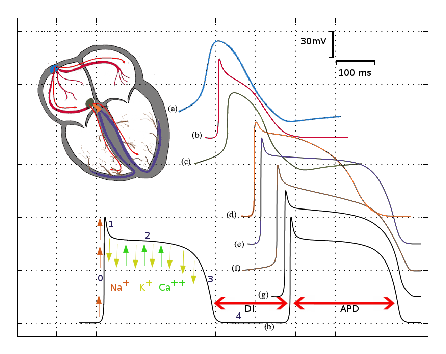
\epsfig{file = ./images/01_chap/APDs2.eps,width = 15cm} 
\caption{Cambio transitorio del voltaje transmembrana, durante un potencial de
acci�n:(a) Nodo sinusal, (b) Auricula, (c) Nodo Auriculo-ventricular (d)
His-bundle,  (e) His-Tawara, (f) Fibras de Purkinje, (g)
Ventriculo (Subendoc�rdico), (h) Ventriculo (subepic�rdico). }
  \label{fig:apds}
\end{figure}


Como se observa en \ref{fig:apds}(h), el \ac{AP} de los ventriculos  presentan
cinco fases distintas, esta caracterizaci�n fisiol�gico comprende:

La fase ascendente del \ac{AP}, es el cambio dr�stico del potencial inicial de
la menbra. En esta fase, conocida como fase 0, la membrana,  de forma
abrupta, permite el ingreso masivo de iones de sodio ($Na^+$) por unos cuantos
segundos.

La  fase de repolarizaci�n inicial, es el instante en que los canales de sodios
se inactivan, y se abren los canales de potasio ($K^+$). En esta fase 1, se
provocando asi una peque�a repolarizaci�n rapida del \ac{AP}, debido a las corrientes de
salida de potasio.

En la siguiente fase, el \ac{AP} se mantiene casi constante (cercano a los 
0mV), y se conoce como fase de meseta o fase 2. En esta fase se activan los
canales de Calcio $(Ca^{2+}$). en esta fase las corrientes de calcio 
son compensadas por las corrientes de potacio, generando el efecto meseta del
\ac{AP}.

En la fase 3, se inactivan los canales de calcio, y s�lo los canales de
potasio quedan activos, permitiendo que el procesos de polarizacion se
accelere. a esta fase se le conoce como fase repolarizaci�n final.

Por �ltimo la el \ac{AP} en estado de reposo, entra a la fase 4, y el potencia
de la menbrana, estable y constante, queda a la espera de un nuevo estimulo que
supere el potencial de umbral, para generar un nuevo \ac{AP}. Al tiempo de
recuperaci�n, que va desde el final del \ac{APD}, hasta el comienzo de un nuevo
\ac{APD}, se loe conoce como \ac{DI}.


El m�sculo card�aco, en condiciones normales, se contrae de acuerdo con los
impulso generados por celular autoexitables, ubicados en algunas zonas del corazon. Dos
nodos autoexitables, que se presentan en la \ref{fig:apds}(a) y (b), son lo 
nodo sinusal y el nodo auriculo-ventricular, respectivamente. Estos dos nodos
tienen la propiedad de despolarizarse de manera espont�nea, es decir no es
necesario la intervenci�n de un est�mulo externos. la \ref{fig:apds}(a) y (b)
refleja como la membrana celular, de dichos nodos,  se despolariza lentamente
durante la fase de reposo debido,principalmente, al cierre gradual de los
canales de potasio y a que la entrada masiva de sodio en el interior de la
c�lula no es tan r�pida como en las celular del ventriculo. Al llegar al
potencial umbral, se da inicio a la despolarizaci�n. en estos nodos se evidencia
la ausencias de la fase de reposo, vista en el \ac{APD} de las c�lulas ventriculares. 


Las c�lulas cardiacas tiene la propiedad de excitabilidad, funcion de \ac{APD}
y del \ac{DI}, y que, en la mayorias de las c�lulas del coraz�n, es
consecuencia de un estimula externos. Pero esta propiedad  de excitabilidad, no
se cumple, por un periodo dentro del tiempo \ac{AP}. El tiempo refractario, o
fase de refractariedad, como se le denomina a este periodo de no exitabilidad,
es el tiempo en el que la celular exitable no responde a un estimula externo,
sin importar su intensidad. 

Por consiguiente, al variar la frecuencia de estimulaci�n del corazon
varia el \ac{DI}. Se estima que el tiempo refractario sea
mayor cuando \ac{DI} es mayor, y viceversa. En consecuencia,
el \ac{APD}, es funci�n tanto del \ac{DI}, como del \ac{APD} predecesor.  El
\ac{APD} dismunuye con la disminuci�n del \ac{DI} y con el incremento en la
frecuencia de estimulaci�n. La relaci�n entre \ac{APD} y \ac{DI} se conoce como
curva de restituci�n, y se observa en \ref{fig:curvares}.

\begin{figure}[t]
\centering
 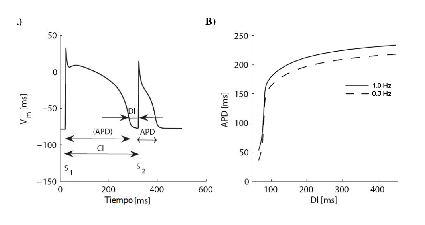
\epsfig{file = ./images/01_chap/curvarestitucion.eps,width = 15cm} 
\caption{Cambio esta curva  esta es vil copia del libro }
  \label{fig:curvares}
\end{figure}

\subsubsection{Sistema de propagaci�n }

El m�sculo cardiaco esta conformado por miocitos y por fibras
musculares. Los miocitos que componen una fibra muscular est� conectados en
serie entre s�, y favorecen la propagaci�n del impulso el�ctrico en la
direcci�n del eje de la fibra muscular. La despolarizaci�n en un miocito, genera
a su vez est�mulos el�ctricos que despolarizan otras celularas vecinas interconectadas electr�camente. 

La principal propiedad del tejido cardiaca  es la propagaci�n del \ac{AP}.
Durrer junto con sus colaboradores en \cite{durrer1970}, presentan el estudio de
la velocidad de propagaci�n del coraz�n humano aislado. Cuando una c�lula es
estimulada, es decir  inicia la despolarizaci�n, la diferencia de potencial
intracelular, aumenta. y por lo tanto, se genera una corriente el�ctrica, entre
la c�lula recien despolarizada  y las c�lula contigua, lo que conlleva al
aumento del potencial interto de la celular vecina. cuando el potencial interno
de la c�lula vecina,  supera el umbrar de desporalizaci�n, dicha celular se
exita. Este proceso se repite con la nueva c�lula, lo que conlleva a la
propagaci�n del \ac{AP} \ac{jalife2011}.

Para la propagaci�n ordenada, en
condiciones normales de un ciclo card�aco, el \ac{AP} es iniciado en el nodo
sinusal, poropagandose por la auriculas. Estas a su vez, estan separadas
electricante  de los ventriculos, y por lo tanto, el \ac{AP} viaja por el nodo
auriculo-ventricular, que conecta el�ctricante las auriculos  con los
ventriculos. El nodo auriculo-ventricular act�an como l�nea de retardo para
lograr una temporizaci�n adecuada entre la acci�n de las aur�culas y
ventr�culo. Una vez terminada la contracci�n de la auriculas, el estimulo  se
propaga desde el has de hiz al sistema de His-Purkinje, desde el cual el
\ac{AP}  se distribuye por el resto de los miocitos  ventriculares. La velocidad
de conducci�n del \ac{AP} depende, principalmente, de la direcci�n en la que se
propaga. el sistema de propagaci�n del \ac{AP} se observar en la parte superior
izquierda de la \ref{fig:apds}, el cual se conoce como tejido especializado de
conducci�n.

Al igual que la dependencia del valor de \ac{APD} con respecto al \ac{DI},  la
propagaci�n del impuso es caracterizado por \acf{CV}. \ac{CV} tambien 
es dependiente de \ac{DI}. En la Figura XXX, se muestra la relaci�n entre el
\ac{CV} y el \ac{DI}. Como se puede observar, y al igual que en el \ac{APD}, la
\ac{CV} disminuye cuando el \ac{DI} disminye, por lo tanto, se dice que a una
tasa de activacion cardiaca mayor, la velocidad de propagacion del est�mulo sera
menor.


\section{M�delo Electrofisiol�gico} \label{sec:modelElectrofi}

Por lo expuesto en la secci�n anterior, se evidencia la actividad
electrofisiol�gica del coraz�n, puede ser  modelada bajos aproximaciones
matematicas, que permiten hoy por hoy realizar estudios cardiacos, por medio de
simulaciones de computador de las diversas dinamicas card�acas. Desde un punto
de vista matem�tico, podemos describir, tanto el flujo de corriente ionicas en
los miocitos, como modelar el sistemas de propagaci�n de \ac{AP}. Como se discution en el apartado
anterior, el aspecto m�s importante de la dinamica del tejido es el \ac{AP}, y 
por lo tanto, los m�delos  electr�fisiol�gicos, principalmente, se basan  en la
simulaci�n del \ac{AP}. Es asi, como existen diversos m�delos computacionales 
electrofisiol�gicos, que se clasifican acorde  a la complejidad asociada a la
representaci�n del funcionamiento del miocardio. Algunos modelos, simulan con
ecuaciones las corrientes ionicas que atreviesan la menbrana celular.

 
Los m�delos matematicos de la membrana celular, que describen el
flujo de corrientes se basan, principalmente, en el 
trabajo desarrollado por Hodgkin-Huxley \cite{Hodgkin52}. este m�delo se observa
en la figura \ref{fig:circuitomembrana}. el m�delo esta  basado en las curvas de corrietne 
nedidas en unsa c�lula nerviosa, por lo cual no se evidencia la contribuci�n de
la corriente de Calcio, que presenta la excitaci�n en los miocitos. en la figura 
\ref{fig:circuitomembrana}, se presenta las contribuciones de las corrientes
generadas por el flujo de sodio ($I_{N_a}$), de potasio ($I_{k}$),  y otros
iones ($I_L (leak current)$). Ademas,  $V_m$,  representa el potencial de
membrana, definido como la diferencia entre los potenciales intracelular
$\Phi_i$ y extracelular $\Phi_e$, por �ltimo $C_m$ refleja el efecto
capacitivo de membrana. El m�delo permite calcular las corrientes i�nicas de
diferente tipo que pasa a trav�s de la membrana del ax�n y el voltaje de
transmembrana. Asi el cambio  de $V_m$ en el tiempo se describe en 
 \ref{eq:N-N}:

\begin{equation}\label{eq:N-N}
\frac{\partial{\mathbf{V_m}}}{\partial{t}}=
\frac{\partial{I_{m} - i_{stim}}}{\partial{C_m}}
\end{equation}

Donde, $I_m$ es la suma de las corriente i�nicas que  atraviesan la
membrana celular,$I_m = I_{Na} + I_K + I_l$ y y $I_{stim}$ representa la
corriente de estimulaci�n aplicada desde el medio extracelular.


\begin{figure}[t]
\centering
 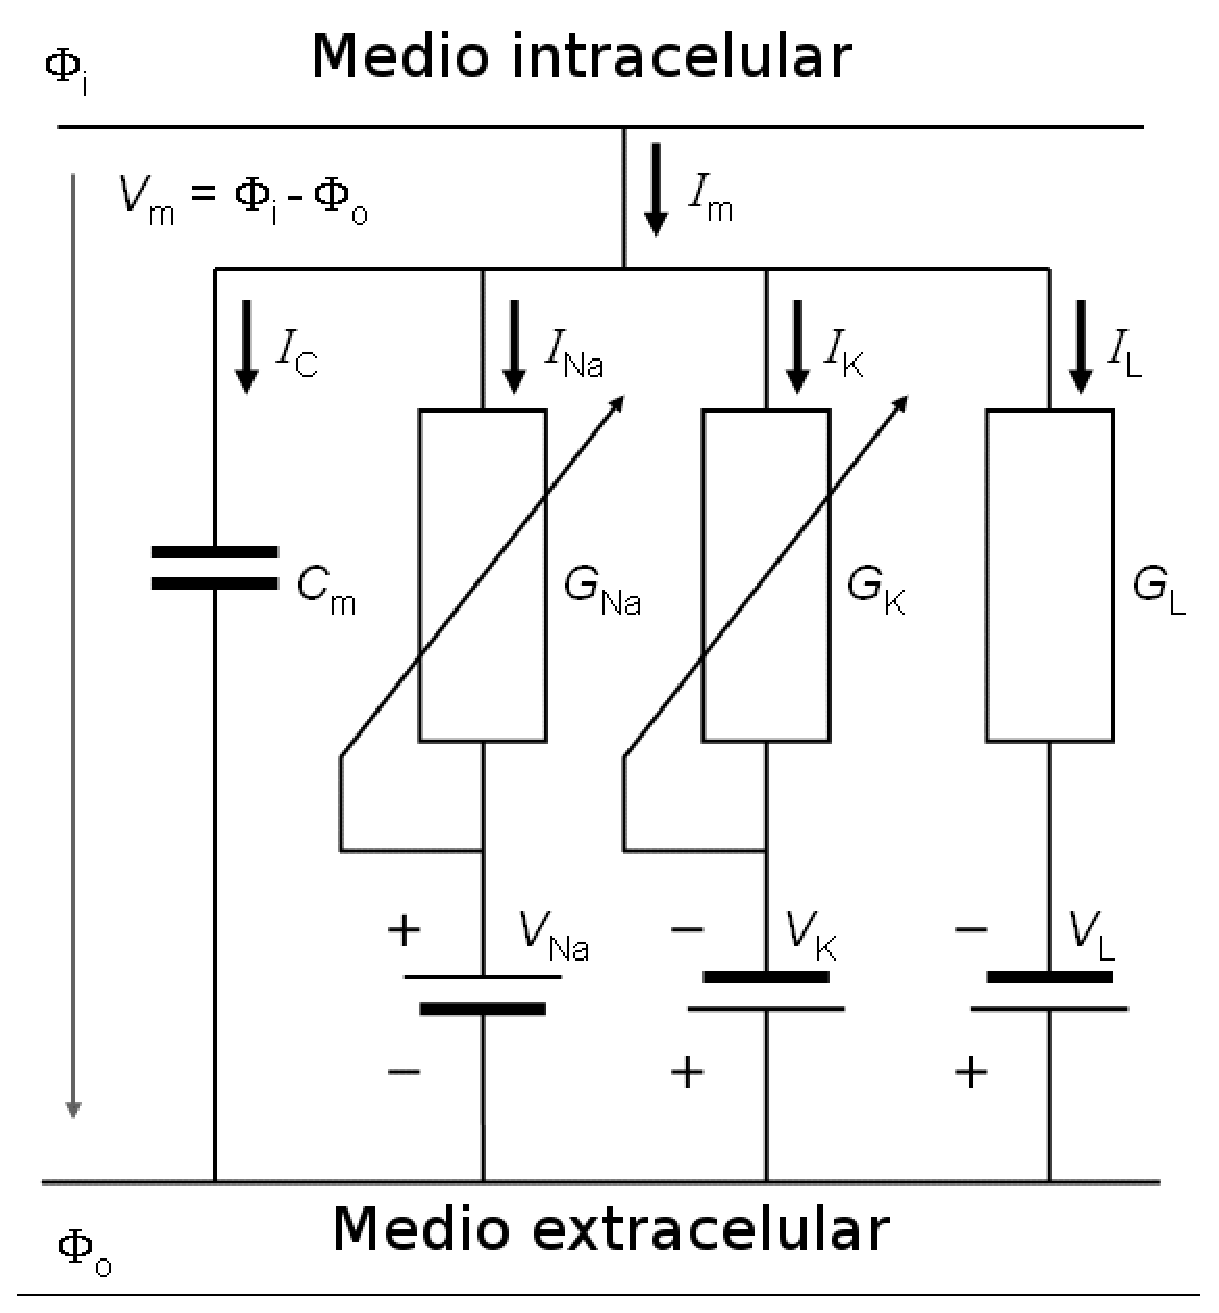
\epsfig{file = ./images/01_chap/circuitomembrana.eps,width = 8cm} 
\caption{Circuito equivalente de la membrana celular Hodgkin-Huxley }
  \label{fig:circuitomembrana}
\end{figure}
 


\subsection{M�delo de la C�lula}

El m�delo de Hodgkin-Huxley, se ha modificado por diversos
autores, permitiendo simular miocitos de zonas especificas del tejido cardiaco,
y con mayor complejida. En \cite{Sachse04}, se compila un listado de diversos
autores, que han modelados los miocitos. Los primeros trabajos basados en
el m�delo de Hodgkin-Huxleym, y que dan inicio al m�delo de c�lulas
cardiacas, en especifico las fibras de purkinje, fueron los trabajo de Noble
\cite{noble1962} y McAllister,R.E \cite{mcallister1975}. 

A posteriori, varios autores proponen diversos m�delo del nodo sinusal en
conejos \cite{noble1984, demir1994}. Por otra parte, las propuestas del m�delo
para los miocitos ventriculares, inician con le trabajo de Beeler y Reuter
\cite{beeler1977}. El planteamiento m�tematico de Beeler y Reutes, es
replanteado en el trabajo de Luo y Rudy \cite{luo1991}. Este �ltimo m�delo, con
las respectivas actualzaciones  y revisiones \cite{luo1994, livshitz2007}, es
posiblemente el mas utilizados hoy en d�a.
Asi mismo en la literatura se encuentran varios autores que han m�delado los
ventriculos de maniferos, como conejos y perros \cite{courtemanche1998,
demir1996, lindblad1996, noble1998}.  El desarrollo del m�delo de la actividad
electrica en venriculos humanos, en los  trabajos de
\cite{nygren1998, bernus2002, sachse2003, ten2004}

En los pr�ximos dos apartados se presenta de manera resumida los
dos m�delos matem�ticos, que son usados en esta Tesis: el m�delo \acf{LRd} y el
aut�mata celular. Ambos m�delos nos permiten generar la actividad
el�ctrica en los miocitos y que posteriormente  son utilizados en la  simulaci�n
del tejidos cardiaco, para generar diversos tipos de arritmias, entre ella la
fibrilaci�n ventricular.  




\subsubsection{M�delo Luo-Ruby}

El m�delo de \acf{LRd}, describe la electrofisiolog�a de un miocito ventricular
del cobayo. el m�delos \ac{LRd}, espresa el formal�smo matematico del \ac{AP} a
partir del desarrollo realizados por Beeler-Reuter \cite{beeler1977}, y aporta
al m�delo la contribci�n de que realza la concentraci�n de calcio $Ca^{2+}$,
en la despolarizaci�n de la celular, voltaje trasnmembrana. Desde publicacion
incial \cite{luo1991}, y luego expandido en  \cite{luo1994}, se han tenido XX 
actualziaciones.  En \cite{zeng1995}, se separa la contribuci�n de las
corrientes de potasio, $I_{Kr}$ y $I_{Ks}$, en contribuci�n rapida y lenta.
a posterior se estudia los efectos de $I_{Kr}$ y $I_{Ks}$  en el \ac{APD}, dando
como resultado la reformulaci�n de la coriente $I_{Ks}$ acorde a tres tipos de
c�lulas diferenten, epicardio, endocardio  y miocardio. este estudio se
encuentra en \cite{viswanathan1999}. Un a�o mas tarde en \cite{faber2000} se 
incluye en el m�delo el formalizmo matem�tico de la corriente generado por el intercambio de
sodio-calcio. Asi mismo, Hund y Rudy en \cite{hund2004}, desarrolaron el
formalismo matem�tico que modelar la electrofisiolog�a de una c�lula ventricular
del perro, \ac{HRd}.

 Livshitz y  Rudy \cite{livshitz2007}  modifican los m�delos \ac{LRd} y
 \ac{HRd}, e incomporan nuevas relaciones entre el transiente de $Ca$, la
 corriente $I_{ca_{(L)}}$. En resumen en la figura \ref{fig:modelHRd}, se
 visualiza el actual m�delo  \ac{LRd} de la celular cardiaca del ventriculo en
 mamiferos,
 
 Como se explico, en la anterior secci�n, hay un gran variedad de  m�delos
 cardiacos para diferentes mamiferos, donde se observan sutiles diferencias
 elctrofisiol�gicas entre las especies, en relaci�n a las corrientes y
 canales ionicos. Entonces a distintos estimulos cada m�delo cardiaco
 tiene un comportamiento diferente, ya que la caracteristicas del \ac{AP}
 varian entre cada especie \cite{OHara2012}, y son de  importnacia en el estudo
 de respuesta a distintos f�rmacos. Sin embargo, esta peque�as diferencias,
 para efectos pr�cticos, en estudios donde trabaja a partir de las propiedades
 macroscopias del \ac{AP} tiende a ser indiferente el tipo de m�delo que sea
 usado. 
  
  \begin{figure}[t]
\centering
 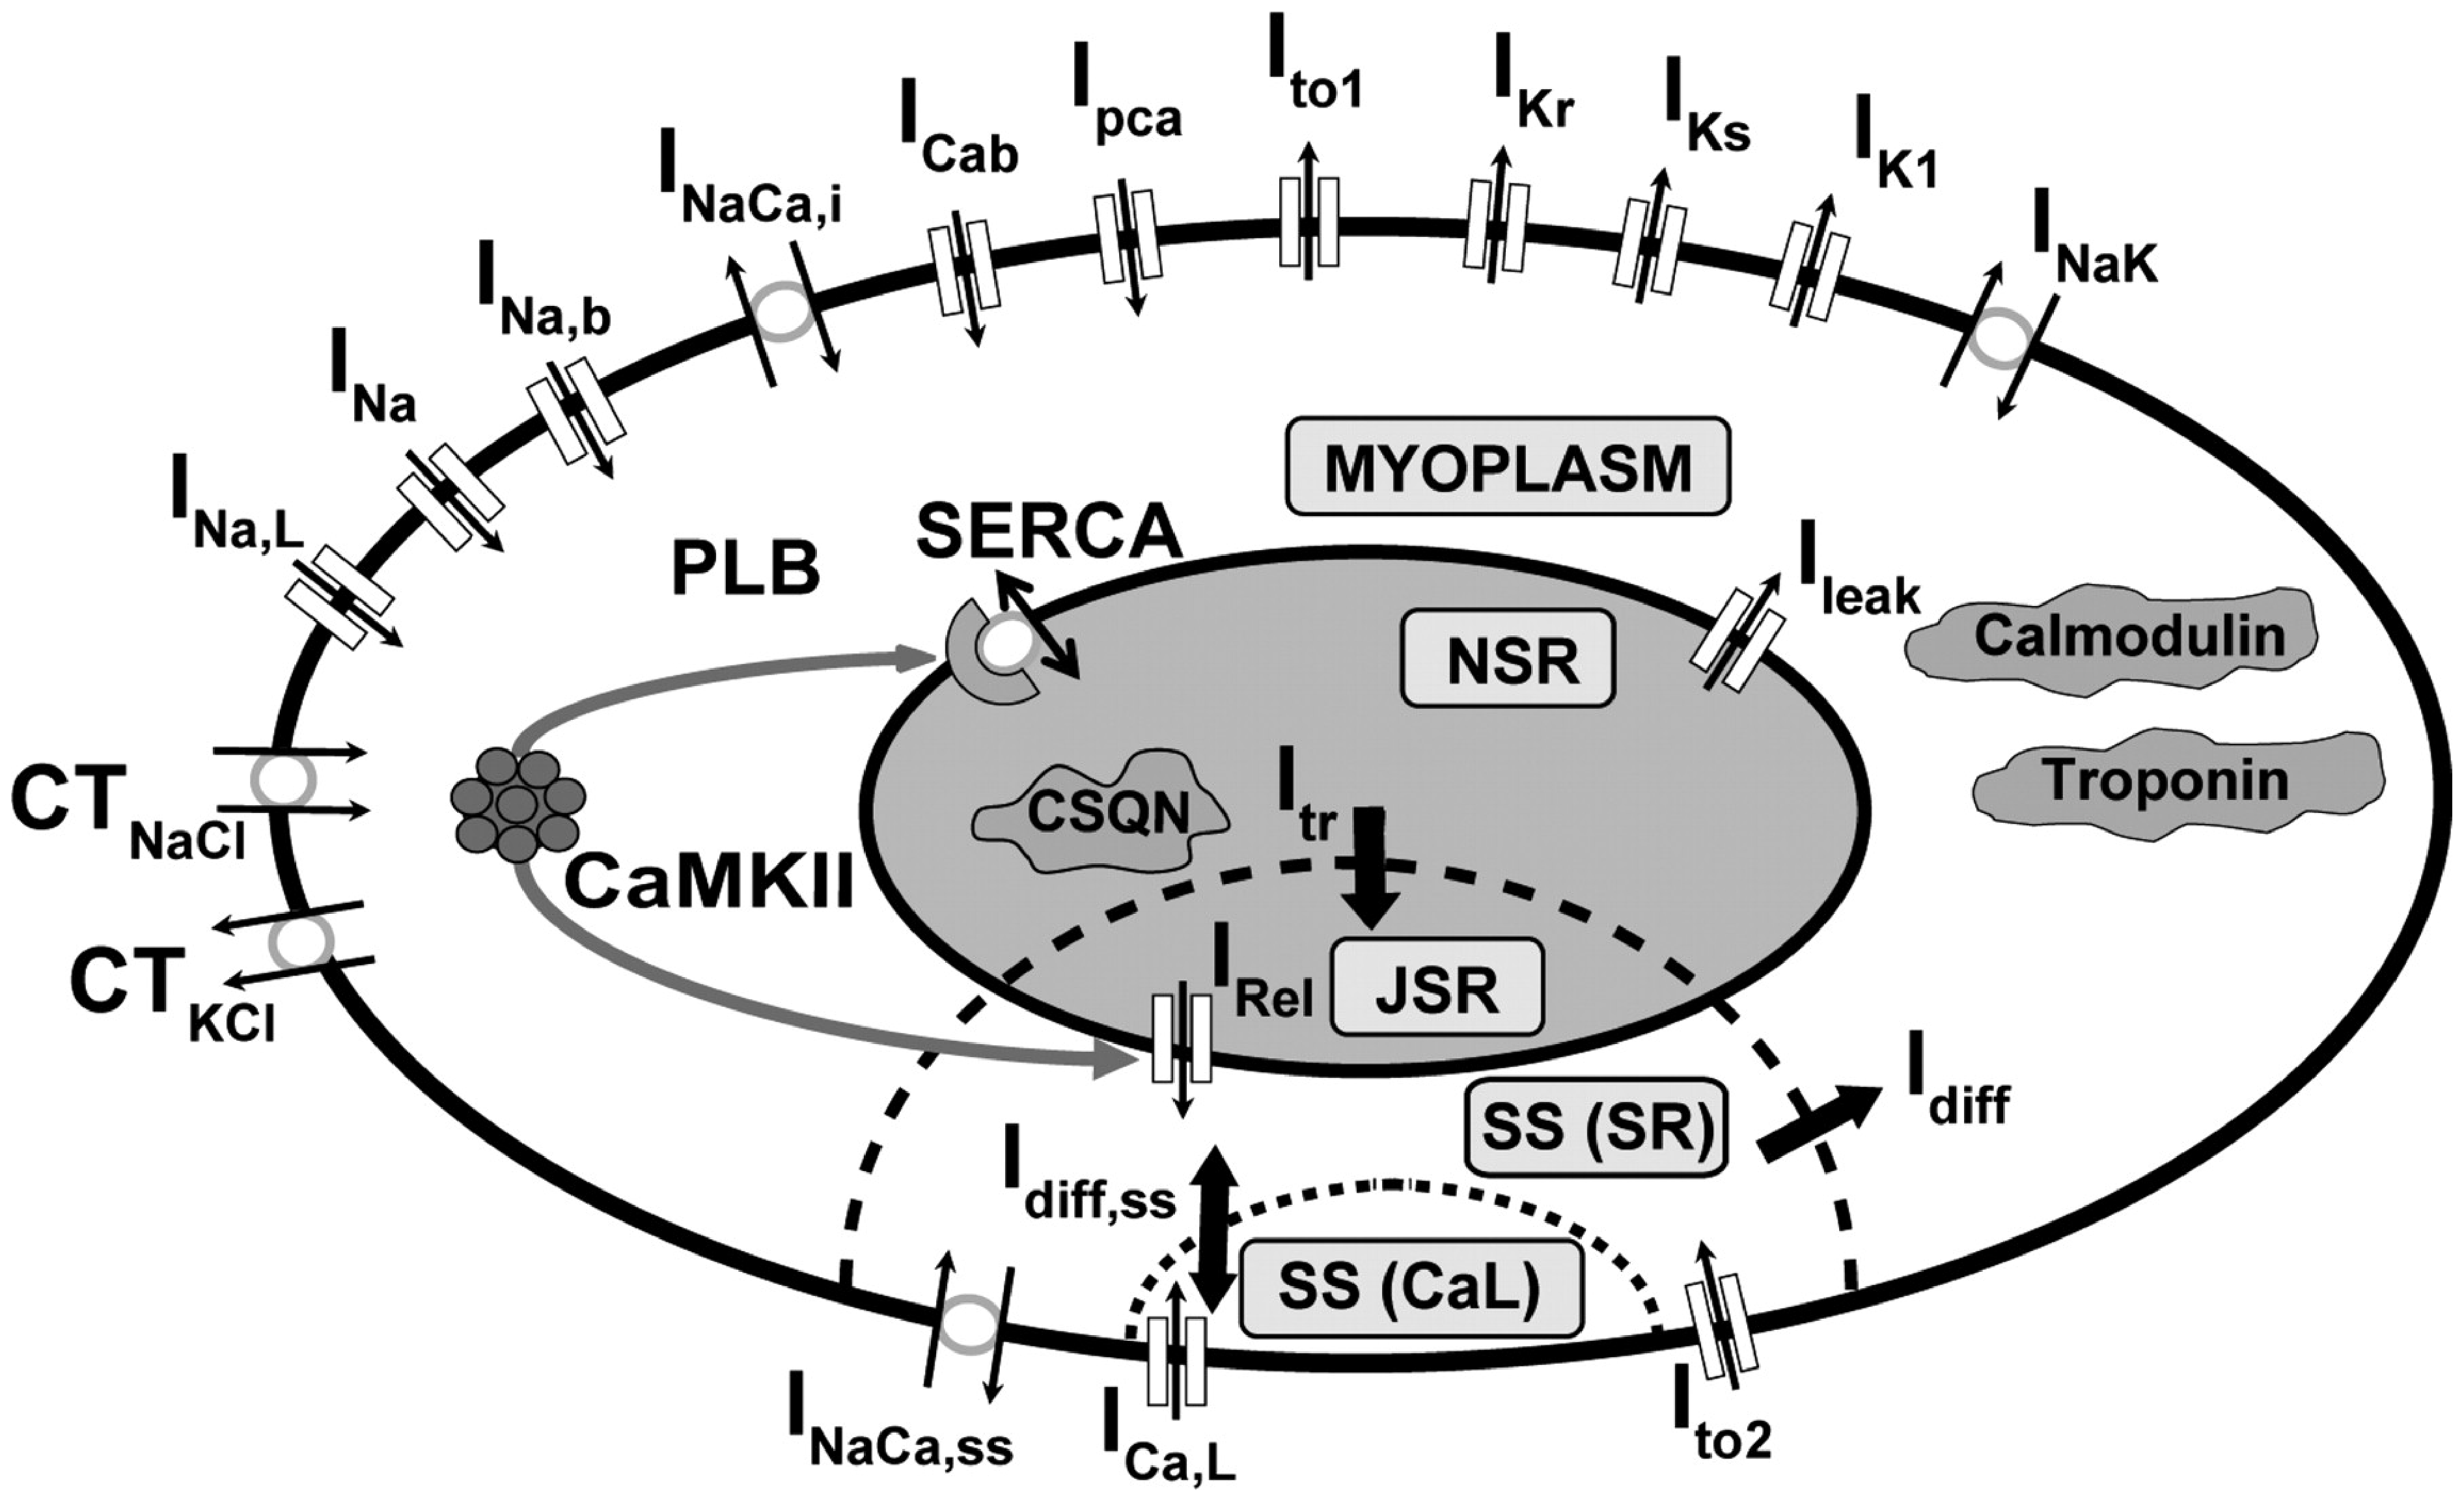
\epsfig{file = ./images/01_chap/modelHRd.eps,width = 10cm} 
\caption{bla bla ). tomado de la web de rudy }
  \label{fig:modelHRd}
\end{figure}

 
\subsubsection{Aut�mata Celular } 


Los aut�matas celulares son ampliamente usados en diversas disciplinas. De igual
maneras, en el contexto de cardiologia celular, un n�mero bastante amplio de
autores han modelado la actividad de la c�lula por medio del aut�mata celular.
La ventaja de utilizar este sistema de \ac{AC}, es la eficiencia
computacional que ofrece la versatilidad de variar las propiedades de conducci�n.

Partiendo de la actividad el�ctrica del miocito,  y principalmente de las
caracteristicas del \ac{AP}, en el \ac{AC}propuesta en 
\cite{Alonso-Atienza05} la celular puede adopta 3 estados diferentes:


\begin{itemize}
\item Reposo: periodo  durante el cual la c�lula esta relaja  y puede ser
estimulada por una fuente externa 
\item Refractario 1: la c�lula se encuentra excitada  y ademas tiene el
suficiente potencial para excitar a c�lulas contiguas.
\item Refractario 2: La c�lula se encuentra excitada, mas sin embargo, el nivel
del \ac{AP} es bajo, y por lo cual pierde la capacidad de excitar a las c�lulas
vecinas.
\end{itemize}

De esta manera, el periodo refractario 1 y 2 es el tiempo  en el cual la c�lula
se encuentras despolarizada, y  por ende la despolarizaci�n del micito, sucede
en la transici�n del estado de Reposo al estado Refractario 1. Por su parte, la
fase 1 de repolalizaci�n parcial de \ac{AP}, debido a las corrientes de salida
del potasio, corresponde a la transici�n del estado Refractario 1 al estado
Refractario 2. La repolarizaci�n total de la c�lula, fase 2, se da en paso del
estado Refractario 2 al estado de Reposo. 


La figura XXXX, muestra las caracteristicas del \ac{AP}. Asi mismo,las
propiedades de restituci�n hacen que el \ac{APD} dependan directamente de la
tasa de estimulaci�n a la que este sometida la membrana celular. Al tener una
frecuencia de estimulaci�n elevada  se observa la reducci�n del \ac{DI}, y como causa, la
reducci�n del \ac{APD}. Sucede lo contrario cuando el ritmo de excitaci�n es
bajo. De esta manera, en el \ac{AC} el tiempo es el estado en reposo es
igual al \ac{DI} y para el \ac{APD}, se fija los tienpo de duraci�n de los
estados refractarios de manera fija, Es decir, el tiempo que permanece
la c�lula es en estado Refractaio 1 es una fracci�n del tiempo total del
\ac{APD}, por lo general el 10\%, y el restatan 90\% es, por lo tanto, el tiempo
que dura la c�lula en el estado refractario 2. Es asi, como los tiempo de
repolaizaci�n total y parcial se fijan acorde al valor de \ac{APD} predecesor.

En cuanto a la despolarizaci�n del micito, en el aut�mata celular se da en
funci�n de la probabilidad de excitaci�n de la c�lula cardiaca. 

falta la figura


\subsection{m�delo de Tejido}

Por lo pronto se ha visto que los m�delos computationales de miocitos card�acos,
han sido herramientas importantes para la comprensi�n del \ac{AP}. y por lo
tanto, para entender los mecanismos que dan lugar a las diferentes arritmias
cardiacas, se han modelados diversas aproximaciones que simulan la propagaci�n
del est�mulo cardiaco. Al igual que los m�delos de celular, los m�delos de los
tejidos cardiacos se agrupan en m�delos microscopicos y macroscopicos. 

los m�delos microsc�picos del tejido del coraz�n, estan restringuidos a
regiones peque�as, debido la alta carga computacional que requiere al tener en
cuenta un elevado numero de variables que contribuyen  tanto en el \ac{AP} como
la velocidad de conducci�n.


\subsubsection{M�delo de la membrana en el aut�mata}

El m�delo \ac{AC} de la membrana esta conformado, como se observa en la Figura
\ref{fig:automata1},  por la red discreta de nodos que representa la estructura
espacial del tejido cardiaco, y en segunda instancia, la representaci�n del \ac{AC} de cada nodo que representan los miocitos. Por lo tanto, se dice que cada miocito,
cuenta con un n�mero $N$ de c�lulas conectadas y de esta forma se
conforma la regi�n de vecindad  usada para  estimar la propogaci�n del \ac{AP}.
la comunicaci�n entre las c�lulas vecinas  es de forma determinista, uniforme  y
sincr�nica.

En esta \nombreDoc, el m�delo del tejido cardiaca, se basa en el 
trabajo realizado en \cite{Alonso-Atienza05}, donde se concibe el musculo
card�aco como un conjunto de elementos (miocitos) discretos interconectados
entre si. Se observa en la Figura \ref{fig:automata1} (a) que el \ac{AP} de
cada c�lula es representada por 3 estados posibles:  Reposo, refractario 1 y 2.
El cambio de  de los estados de cada c�lula, viene dado en funci�n del estado
de los elementos vecinos y de  acuerdo al estado predecesor. El valor de voltaje
de la membrana, es prototipado a partir del modelo \ac{LRd}
\cite{Alonso-Atienza05}



  \begin{figure}
\centering
 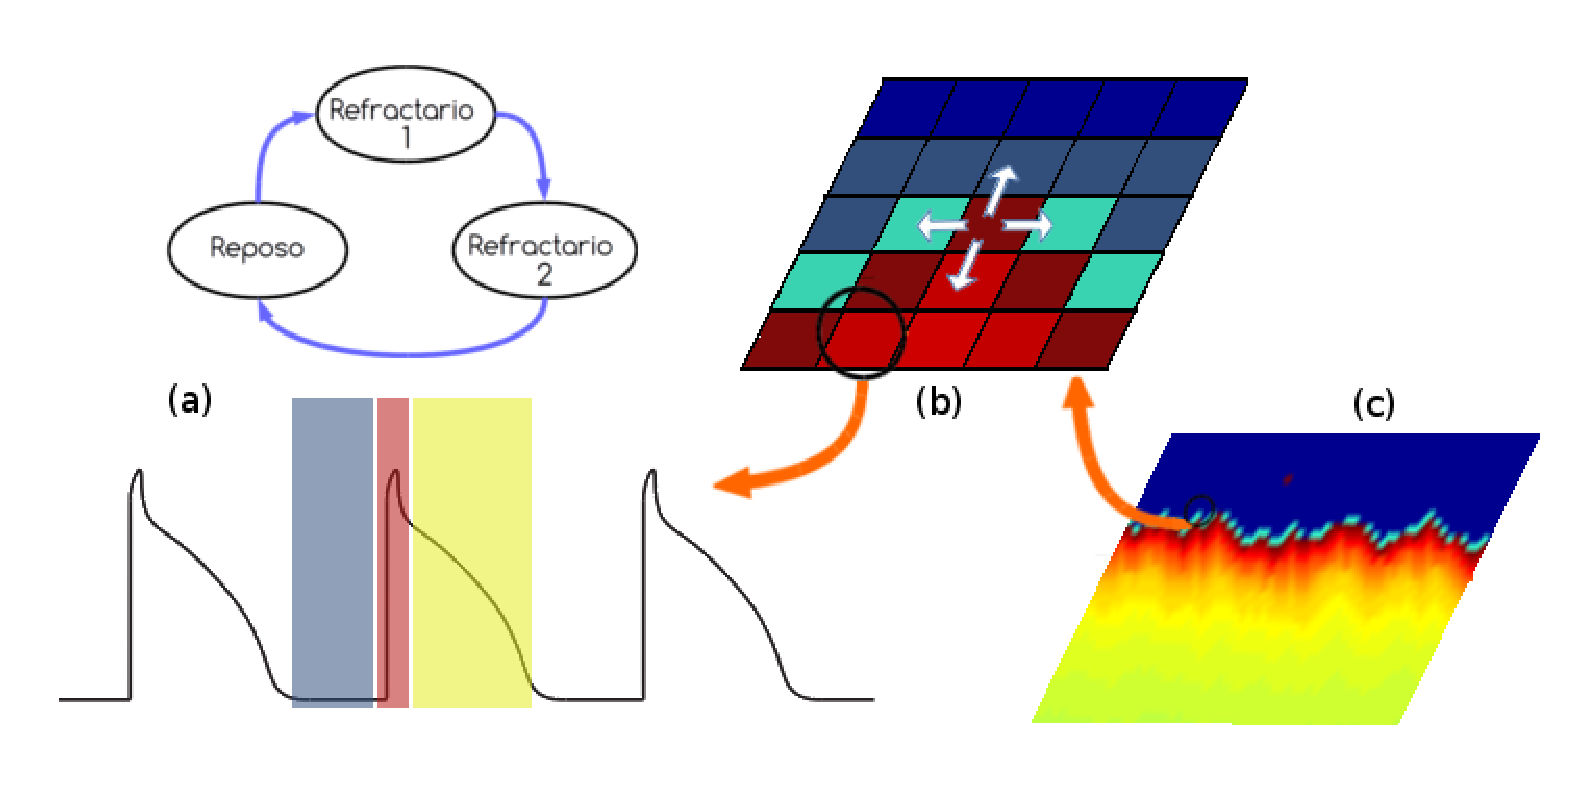
\epsfig{file = ./images/01_chap/automata1.eps,width = 14cm} 
\caption{Represetaci�n del m�delo del aut�mata celular. (a)Prototipo de \ac(AP)
con niveles de $V_m$. el nivel de $V_m$ se asocia a los tres estados del
automata definidos en \cite{Alonso-Atienza05} (b) Cada celda esta modelada por
medio del aut�mata celular, que se conecta con 4 vecinos, la vecinda  tiene forma de cruz  y esta commpuesta por 5 celdas. (c) representaci�n de la
propagacion del \ac{AP} en un tejido de 100x100 celdas.}
  \label{fig:automata1}
\end{figure}

En la propagaci�n del \ac{AP}, la despolarizaci�n de la c�lula, en el modelo
\cite{Alonso-Atienza05}, se define en terminos probabil�sticos y , se tienen en
cuenta el grado de excitabilidad de la c�lula (E) y la cantidad de celdas
exitadas de la vecindad (Q). Por lo tanto, si ${P_{j}}^{exc}$ es la
probabilidad de excitaci�n de la c�lula, decimos:

\begin{equation}\label{eq:Propaga}
P_j^{exc}= k\cdot E\cdot Q
\end{equation}

Donde $k$, es una constante de proporcionalidad. $E$ viene determinda por las
curvas de restituci�n de \ac{CV} y $Q$ es definida en funci�n del n�mero de
c�lulas que se encuentran en estado Refractario 1. Por lo tanto, al aumentar
\ac{CV} la ${P_{j}}^{exc}$ de la c�lula $i$ aumente, y de igual manera, sucede
si se aumenta el n�mero de c�lulas vecinas recien estimuladas.

Cada c�lula en el automa celular tiene la capacidad de excitar a las
c�lulas vecinas s�lo cuando dicha c�lula se encuentra en el estado
Refractario 1. Se codifican los estados de la c�lula en (A):
1 cuando la c�lula esta en estado refractario 1 y, 0 si la
c�lula ha perdido la propiedad de excitar a otras c�lulas
\cite{Alonso-Atienza05}, por lo tanto, $P_j^{exc}$ esta definida por:


\begin{equation}\label{eq:Propaga2}
P_j^{exc}= k \cdot E\cdot\sum_{i \neq j}\frac{A_i}{d_{ji}^2}
\end{equation}

Donde $i$ indica una celda pertenecientes a la vecindad de la c�lula $j$. $A_i$,
representa la codificaci�n de los dos estados de la c�lula, (1 o 0) y $d_{ji}$ 
es la distancia de conexi�n entre la celda $i$ y la celda $j$.


Aca seria bueno poner como se generan las dinamicas variando cv y apd, eso lo
tengo yo ahi en el computador de la sun,,, de esta forma validamos el uso de
este automata para la tesis

Por lo tanto, se puede hablar que el m�delo del mu�culo cardiaco, a trav�s de
\ac{AC}, es una simplificaci�n del tejido cardiaco, que permite  simular las
propiedades de propagacion del \ac{AP}.


\subsubsection{m�delo de reaccion-difusi�n}

Los m�delos reaccion-difusi�n para representa la din�ica del tejido cardiaco,
por un lado modelan la conexi�n  entre las c�lulas a partir de
resistencias el�ctricas y, por otro lado la actividad el�ctrica de la c�lula es
reproducica con la simulaci�n de los canales  y corrientes i�nicas. A primera
instancia se observa que este tipo de mod�lo es mucho mas realistas y por lo
tanto, la dinamicas cardiacas complejas son reproducidas de mejor manera.

Los sistemas de reacci�n-difusi�n, utilizan ecuaciones diferenciales no lineales
para describir el proceso de excitaci�n de la celular y propagaci�n.

\begin{equation}\label{eq:r-d}
\frac{\partial{u_i}}{\partial{t}}=f_i(u_i, \ldots,u_n) + \nabla \dot
(\mathbf{D}_i \nabla u_i), i=1,\ldots.n
\end{equation}

Donde $u_i$ es la variable de estado, para el caso del tejido cardiaco $u_i$
represtna la diferencia de potencial de la transmembrana, la conductividad de
los canales  y la concentraci�n i�nica \cite{Sachse04}. $f_i$ es el grado de excitaci�n, y
$\mathbf{D}_i$ el tensor de difusi�n. a su vez el cambio de estado es
determinado por $f_i$ y $\nabla \dot(\mathbf{D}_i \nabla u_i)$

Para el musculo cardiaco, se considera que el tejido se comporta
como un sistema compuesto por tres medios continuos \cite{holden1997}, el medio
intrecelular, el medio extracelular y la membrana celular. lo que conlleva a
representar las celulas electrofisiol�gicas con la aproximaci�n de dos modelos
el modelo bidominio y el modelo momodominio.


Estos dos modelos, el bidominio  y monodominio, combinan los
modelos electrofisiol�gios, con el flujo de corriente a trav�s de los espacios
extracelulares y/o intracelulares, respectivamtente. Como se observa en la
figura \ref{fig:mono_bidominio}, este enfoque biofisico, une el modelo de
menbrana celular con el modelo de corrientes, este �ltimo modela el acoplamiento
el�ctrico de la conductividad de membrana celular con el medio, a trav�s de
resistencias. La diferencia de los modelos bidominos y monodominos, es por lo
tanto, el n�mero de dominos que maneja el modelo, para el flujo de la corriente
el�ctrica.

El modelo monodominio incorpora los efectos de la conductancia
intracelular, y asume que la diferencia de potencial entre el medio extracelular  y la
menbrana es cero. en otras palabras el potencial de membrana $V_m$, es equivalente al
potencia intracelual $\theta_i$. tomando la ecuaci�n \ref{eq:r-d}




[ 242 , 243 , 244 ] o tensores de conductividad . En cada
paso de tiempo y para cada celda se realizan dos c�lculo


En el modelo bidominio \cite{henriquez1992, miller1978}, el tejido cardiaco est�
compuesto por dos medios continuos, uno intracelular y otro extracelular que ocupan el
mismo espacio f�sico. el medio intracelular representa el interior de la c�lula,
mientras que el medio extracelular modela el espacio entre c�lular. se habla de
que los espacion son continuosm en el sentido  que las corrientes pueden fluir
de una c�lula a otra, a trav�s del medio intracelular (debido a las uniones
comunicantes), sin tener que pasar por el medio extracelular. 


\begin{figure}
\centering
 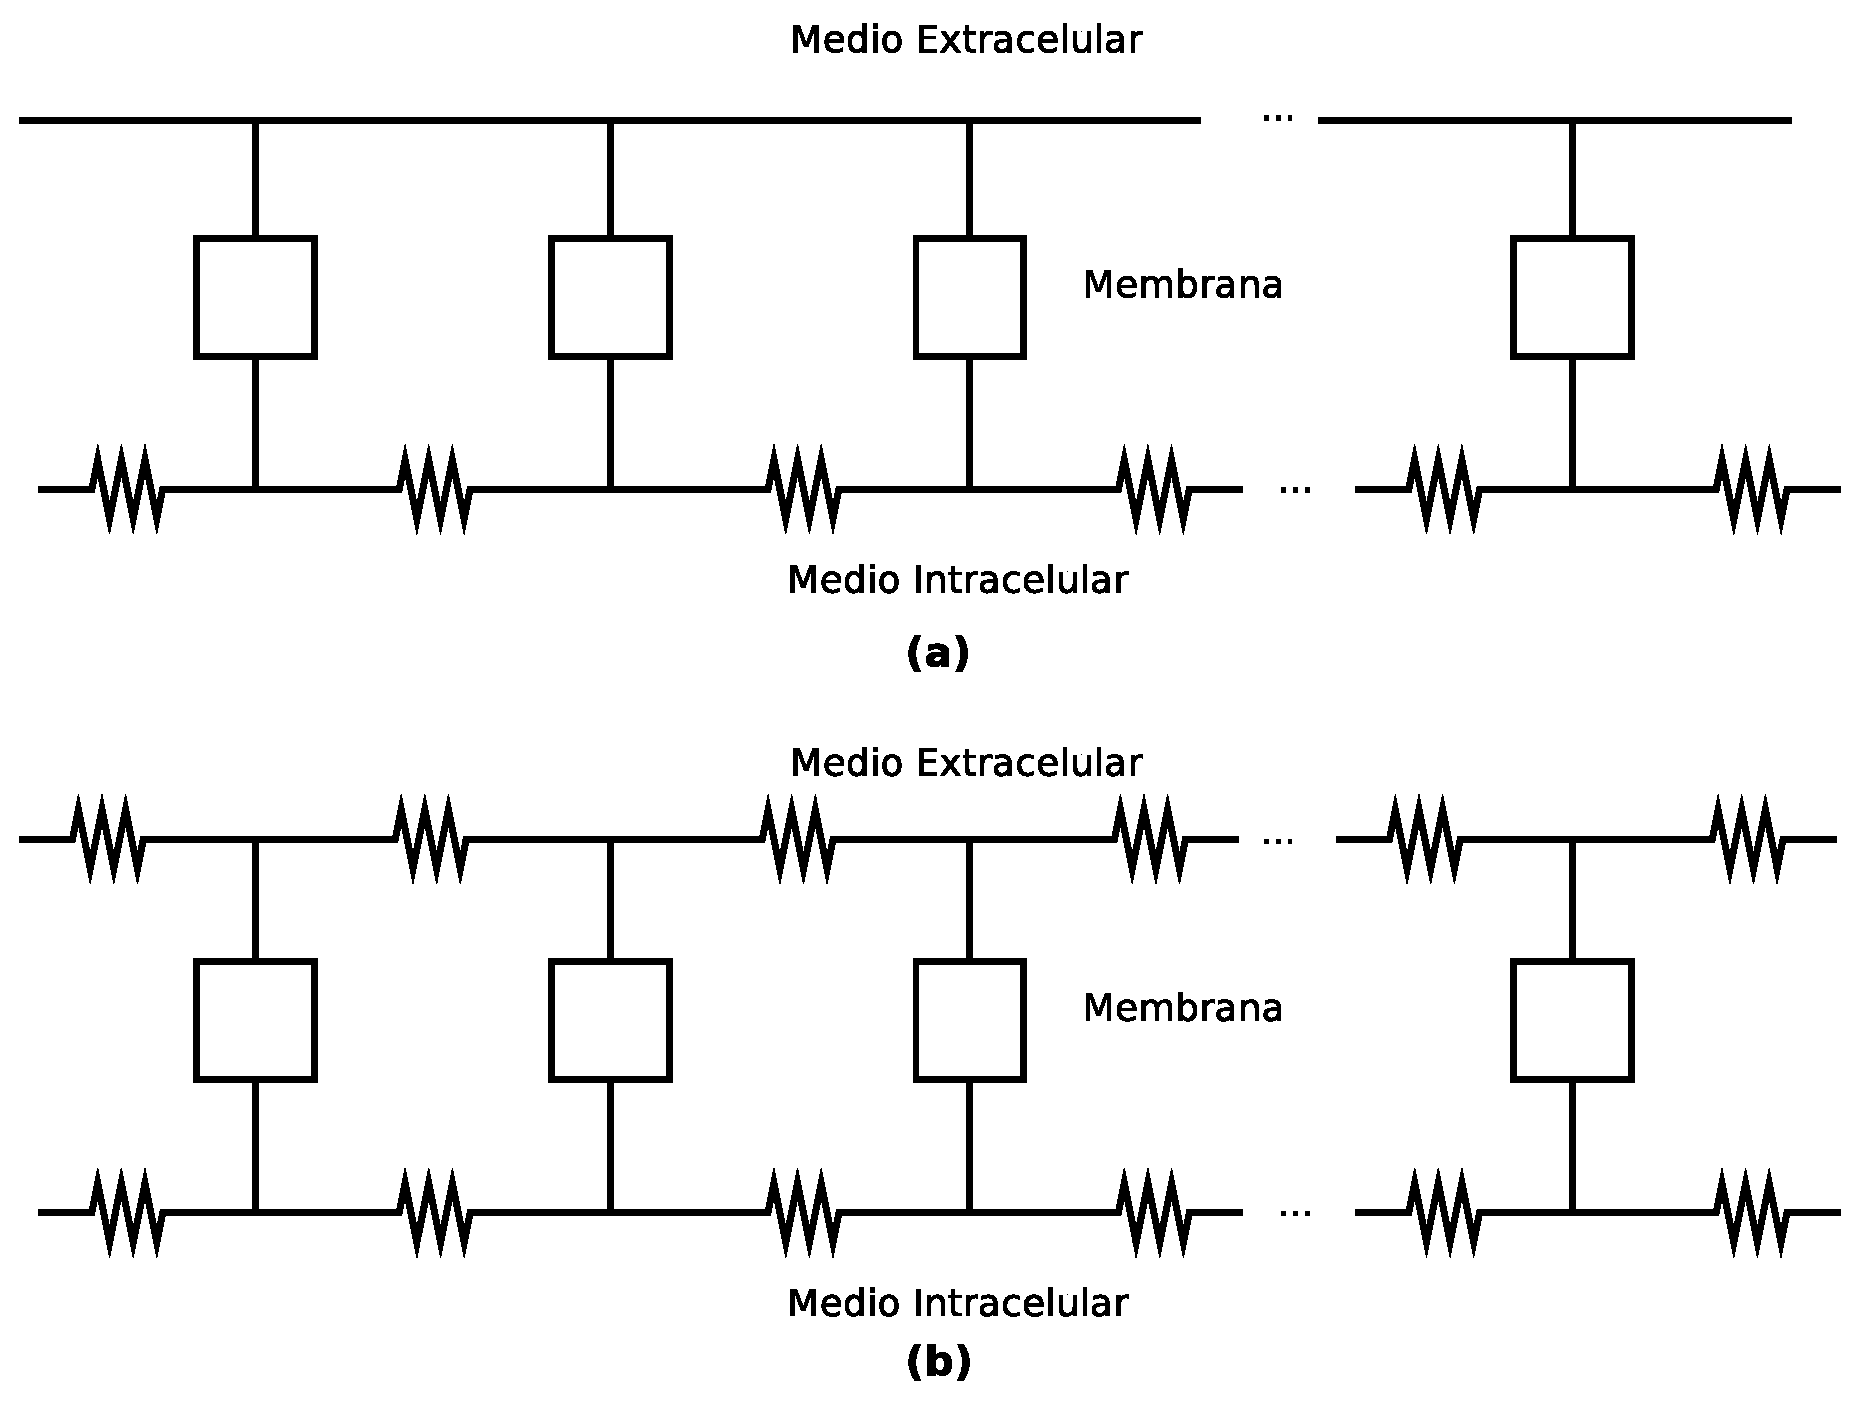
\epsfig{file = ./images/01_chap/modelosbiofisicos.eps,width = 14cm} 
\caption{Diagrama del modelo de tejido unidimensional simulado. Modelos
circuitales biof�sicos: (a) monodomino y (b) bidominio}
  \label{fig:mono_bidominio}
\end{figure}



no se que poner aca si las ecuaciones o dejar aca  y ya  y hablar mas bien de
lso modelso 2d  y 3d


\section{Sistemas de medida}
algo de ac� http://www.bem.fi/book/ \cite{Malmivuo95}


The excitation propagation process can be registered with extracorporal
electrodes


Cardiac sources are the bioelectric processes generated by the heart during
contraction. There exist different, equivalent mathematical paradigms to model
the activity of cardiac sources, such as the monopole field and the dipole
field \cite{Malmivuo95}. In this study, we model cardiac sources as a
time-varying dipole field, i.e. as a spatial distribution of time-varying
dipoles $\mathbf{J}(v,t)= [J_x(v,t), J_y(v,t), J_z(v,t)]^T$ on a volume $V$,
where $v$ denotes a point located inside $V$ and $t$ denotes the time instant.

 The time-varying activity of cardiac sources can be measured by lead systems,
 producing cardiac signals. Taking the dipole field as our reference description
 for cardiac sources, we follow a lead-field approach to model cardiac signals
 \cite{Malmivuo95}. According to the lead-field theory, the cardiac signal
 $c(t)$ that is induced at a lead system by a dipole field $\mathbf{J}(v,t)$ can
 be expressed as

\begin{equation}\label{eq:EqSintesis}
c(t)=\int_V{\mathbf{L}^{T}(v) \mathbf{J}(v,t)}{dv}
\end{equation}

 where the vector field $\mathbf{L}(v)= [L_x(v), L_y(v), L_z(v)]^T$ is the
 measurement sensitivity distribution (MSD) and describes the ability of the
l ead system to measure cardiac dipoles located at $v\in V$. In words, cardiac
si gnals are a weighted linear combination of the underlying cardiac sources.



\subsection{Sistema de Electrodos}
definici�n de las ecuaciones lapalaciano
\subsection{Volumen equivalente de sistema de electrodos}
 \ac{LF}


\section{Conclusiones}


% -*-coding: iso-latin-1  -*-
\chapter{Definici�n  del Espectro}



\begin{resumen}


En el siguiente cap�tulo se aborda el formalismo matem�tico que enmarca el
estudio del espectro de las se�ales cardiacas de esta \nombreDoc, y el cual se
encuentra en la publicaci�n \cite{Requena13b} . El objetivo del capitulo es desarrollar  la
teor�a que conecta el espectro de la se�ales cardiacas, con su din�mica espacio-temporal.
Por lo tanto, los resultados te�ricos, presentes  en este capitulo, derivan en
el an�lisis e interpretaci�n del espectro de se�ales cardiacas, que se
contemplan en el pr�ximo cap�tulo

La relaci�n entre los diferentes sistemas de mediada de se�ales cardiacas y los
espectros de las mismas, se abordar a partir del an�lisis de se�ales
multivariantes junto con m�delos bioel�ctricos. A su vez, se definen mapas de
autocorrelaci�n para las fuentes  y se�ales  bioel�ctricas, de esta forma, de
acuerdo con la correlaci�n espacio-temporal, se clasifican las diferentes
din�micas cardiacas, en perfectamente correlacionandas, parcialmente
correlacionadas  y perfectamente incorrelacionadas. A si mismo, se abordan los
diferentes m�todos de estimaci�n del espectro de se�ales.

Para terminar, se aborda los mapas de (\ac{DF}), como ejemplo de an�lisis
espectral. en donde se expome la relaci�n entre las caracteristicas del sistema
de electrodos, utilizados para estimar la actividad local del miocardio, y el
ancho de banda del espectro resultante.

tesis de jesus  en resumen  y lo del articulo la parte te�rica

llega hasta la descrip la correlaci�n de voltajes  definicion de tipos de
fuentes se toma del articulo

medidad del grado de correlaci�n espacio temporal



\end{resumen}


\section{Introducci�n}

Los procesos estoc�sticos nos permiten modelar aquellos sistemas
multivariantes, en tiempo y espacio. De esta manera, gracias a las herramientas
estadisticas, se puede estudiar como se comportan se�ales variantes en el
tiempo, que de otra forma serian muy dificiles de tratar.

Una variable aleatoria, como funci�n medible que asigna un n�mero real a cada
posible resultado del espacio muestral de un experimento aleatorio, se
puede caracterizar por medio de su probabilidad de ocurrencia. De esta forma, la
funci�n de distribuci�n ${F(x)}$  es una descripci�n de las probabilidades asociadas a los posibles
valores de la variable aleatoria. 

Por tanto, toda variable aleatoria tiene asociada una funci�n de distribuci�n
${F(x)}$, tal que ${F(x)=P(X \leq x)}$. Para variables aleatoria continua, la 
distribuci�n de probabilidad viene descrita por una funci�n de densidad
${f(x)}$. en donde, ${f(x)= dF(x)/dx}$. Asi mismo,  para las variables
aleatorias discretas relacionamos la funci�n de distribuci�n con la funci�n de
densidad como ${F(x)= \displaystyle\sum_{x_i \leq x }f(x_i)}$.

Un proceso estocastico es una sucesi�n infinita de variables aleatorias que
evolucionan en el tiempo. Por lo tanto, al dependen del un tiempo
$t$  la funci�n de distribuci�n da lugar a ${F(x,t)=P(\mathbf{x}(t) \leq x)}$.
Por lo que, la funci�n de densidad de $x(t)$ es $f(x,t)=
\partial{F(x,t)}/\partial{x}$ \cite{Papoulis91}.

Los modelos estoc�sticos son fundamentales para el an�lisis espectral de se�ales
biolectricas, y en general en se�ales discretas que se analizan en un tiempo
finito. De esta formas, tanto la autocorrelaci�n con la densidad espectral de
potencia, son habitualmente muy utilizadas para describir procesos
estocasticos de segundo orden. Con los estadisticos de segundo orden, por lo
tanto, es posible describir patrones, tales como la periidicidad  y la
coherencia de las se�ales \cite{Requena08}.

\subsection{Correlaci�n de Se�ales}\label{subs:corresignal}
Siendo $\mathbf{x}(t)$, un proceso estocasticos real y $\mathbf{x}(t_1)$,
$\mathbf{x}(t_2)$, dos valiables aleatorias, se define, $\mathbf{R}(t_1,t_2)$,
la autocorrelaci�n de $\mathbf{x}(t)$ como \cite{Papoulis91}:

\begin{eqnarray}\label{eq:autocorrelation}
	\mathbf{R}(t_1,t_2)=E{\{ \mathbf{x}(t_1)\mathbf{x}(t_2) \}}
\end{eqnarray}
Donde $E$ es la media estadistica. De esta manera, se define la autocorrelaci�n
de un procesos $\mathbf{x}$, real o complejo, como la media estadistica del
producto de $\mathbf{x}(t_1)\mathbf{x}^*(t_2)$, donde la m�xima correlaci�n se
obtienen cuando $t_1=t_2$.

Cuando se tiene dos procesos estocasticos $\mathbf{x}(t)$ y
$\mathbf{y}(t)$,se habla de corelaci�n cruzada $\mathbf{R}_{xy}(\tau)$. como 
\cite{Requena08}:

\begin{eqnarray}\label{eq:correlation}
	\mathbf{R}_{xy}(\tau)=E{\{ \mathbf{x}(t-\tau)\mathbf{y}(t) \}}
\end{eqnarray}
De esta forma, la correlaci�n es la operaci�n b�sica para la b�squeda de
patrones por emparejamiento. como se expone en \cite{Requena08} el ruido blanco,
$W(t)$, es un porcesos estoc�stico particular cuya funci�n de autocorrelaci�n es
$\mathbf{R}(\tau)= \delta(\tau)$, donde $\delta(\tau)$ es la funci�n delta de
Dirac, y lo que indica es que las variables aleatorias que conforman $W(t)$
no estan correlacionadas entre si.


\subsection{Correlaci�n de Vectores}\label{subs:correvector}

Un procesos vectorial, de $n$ dimensiones, es una familia de $n$ procesos
estocasticos. Por lo tanto, un proceso estoc�stico vectorial es un
vector cuyas componentes son procesos estoc�sticos escalares \cite{Requena08}. 

Se extienda la definici�n de la correlaci�n de dos se�ales, secci�n
\ref{subs:corresignal}, a los procesos vectoriales, al realizar para cada par de
procesos escalares  definidos por el producto vectorial de dos procesos
vectoriales, como se expone en \cite{Requena08}. La correlaci�n de vectores es la correlaci�n cruzada de los
componentes del vector que dan como resultado las matriz de correlaci�n
cruzada.

Si $\mathbf{V}_n(t)$ y $\mathbf{W}_n(t)$ son dos procesos vectoriales  de $n$
dimensiones, $\{v_1, v_2, v_3, \ldots v_n\}$ y  $\{w_1, w_2, w_3, \ldots
w_n\}$ los respectivos procesos estocasticos. Entonces, acorde con la
la ecuaci�n \ref{eq:correlation}, decimos que la correlaci�n cruzada entre dos
componentes de $\mathbf{V}_n(t)$ y $\mathbf{W}_n(t)$, esta definida 

 \begin{eqnarray}\label{eq:correlationCompVector}
 {\rho_{11}}(v,w,\tau)=E{\{ \mathbf{v_1}(t-\tau)\mathbf{w_1}(t) \}}
 \end{eqnarray}

De esta forma, la matriz de correlaci�n cruzada entre dos procesos vectoriales
$\mathbf{V}_n(t)$ y $\mathbf{W}_n(t)$, se define 

 \begin{eqnarray}\label{eq:correlationVector}
 &&\boldsymbol{\rho}(v,w,\tau)
 = \left( \begin{array}{cccc}
 {\rho}_{11}(v,w,\tau) & {\rho}_{12}(v,w,\tau) & \ldots &{\rho}_{1n}(v,w,\tau)\\
 {\rho}_{21}(v,w,\tau) & {\rho}_{22}(v,w,\tau) & \ldots &{\rho}_{2n}(v,w,\tau)\\
 \ldots & \ldots& & \ldots\\
 {\rho}_{n1}(v,w,\tau) & {\rho}_{n2}(v,w,\tau) & \ldots &{\rho}_{nn}(v,w,\tau) 
 \end{array} \right).
 \end{eqnarray}
 

Si  $\boldsymbol{\rho}(v,w,\tau)$  es una matriz  nula de $nxn$ elementos, se
decir que los dos procesos vectorales estas incorrelacionados. Adicionalmente,
si $\mathbf{V}_n(t) = \mathbf{W}_n(t)$, entonces hablamos de que la diagonal de la
matriz $\boldsymbol{\rho}(v,w,\tau)$, es la autocorrelaci�n de cada una de las
componestes del  proceso vectorial.


\section{Autocorrelaci�n de fuentes bioelectricas}

En esta secci�n nosotros proponemos la definici�n de autocorrelaci�n tanto de
fuentes como de sen�ales cardiacas. Nuestro punto de partida se refleja del
trabajo realizado en \cite{Requena08}, que junto con la
definici�n de dipolo bioel�ctrico de la secci�n \ref{sec:modelElectrofi}
enmarcan las fuentes bioel�ctricas en los procesos estocasticos de segundo.


\subsection{Autocorrelaci�n  de fuentes cardiacas}

Como se vio en la secci�n \ref{sec:modelElectrofi}, nosotros tomamos el dipolo
cardiaco como elemento basico de una fuente cardiaca, y de esta forma definimos
la autocorrelaci�n de fuentes cardiacas, como la correlaci�n cruzada entre un
dipolo cardiaco y todos los dipolos pertenecientes al tejido.

El dipolo cardiaco es un ente  vectorial, tal que $\mathbf{J}(v,t)={\{ J_x(v,t),
J_y(v,t), J_z(v,t) \}}$ \cite{Malmivuo95}, por lo que podemos extrapolar la
correlaci�n de vectores de  \ref{subs:correvector} a la correlacion entre dos
dipolos,  como la correlaci�n cruzada entre las tres componentes de cada dipolo.

La media de un dipolo cardiaco, segun \cite{Papoulis91},  esta dada por:
  
 \begin{eqnarray}\label{eq:average_dipole}
 \bar{\mathbf{J}}(v)&=&\langle\mathbf{J}(v,t)\rangle_t  \nonumber \\
	&=& [\langle J_x(v,t)\rangle_t, \langle J_y(v,t)\rangle_t, \langle J_z(v,t)\rangle_t]^T. 
 \end{eqnarray}

A continuaci�n  y basados en  $\bar{\mathbf{J}}(v)$, se define el dipolo
cardiaco con media cero, $\langle\mathbf{J'}(v,t)\rangle_t=\mathbf{0}$, como:


\begin{eqnarray}\label{eq:zero_average_dipole}
	\mathbf{J'}(v,t)=\mathbf{J}(v,t)-\bar{\mathbf{J}}(v)
\end{eqnarray}

La correlaci�n cruzada entre dos dipolos cardiacos, $\mathbf{J}(v,t)$ y 
$\mathbf{J}(w,t)$, del tejido cardiaco definido por $V$, queda definida como:

 \begin{eqnarray}\label{eq:autocorrelation_source}
 &&\boldsymbol{\rho}(v,w,\tau)=\langle\mathbf{J'}(v,t+\tau)\mathbf{J'}^{T}(w,t)\rangle_t
 \nonumber \\
 &&= \left( \begin{array}{ccc}
 {\rho}_{xx}(v,w,\tau) & {\rho}_{xy}(v,w,\tau) & {\rho}_{xz}(v,w,\tau) \\
 {\rho}_{yx}(v,w,\tau) & {\rho}_{yy}(v,w,\tau) & {\rho}_{yz}(v,w,\tau) \\
 {\rho}_{zx}(v,w,\tau) & {\rho}_{zy}(v,w,\tau) & {\rho}_{zz}(v,w,\tau) 
 \end{array} \right).
 \end{eqnarray}

Donde, $\boldsymbol{\rho}(v,w,\tau)$, define la matriz  que describe la
correlaci�n cruzada entre cada una de las componentes del par de dipolos, 
$\mathbf{J}(v,t)$ y $\mathbf{J}(w,t)$ del  tejido cardiaco. 

Ahora bien, para definir la autocorrelaci�n de fuentes cardiacas,  nosotros
definimo es primera instancia, a partir de \ref{eq:autocorrelation_source}, la
correlaci�n cruzada  total  entre dos dipolos cardiacos $\mathbf{J}(v,t)$ y
$\mathbf{J}(w,t)$, como la suma de todos los elementos de $\boldsymbol{\rho}(v,w,\tau)$.

\begin{eqnarray} 
  R_{J}(v,w,\tau) &=&  \mathbf{1}^{T} \boldsymbol{\rho}(v,w,\tau) 
  \mathbf{1},\label{total_corr}
\end{eqnarray}



Para normalizar la correlaci�n cruzada total es necesario definir la potencia
media del dipolo cardiaco como:

\begin{equation}\label{eq:Potencia}
{P}(v) = {R_{J}}(v,v,0)
\end{equation}

Donde, ${R_{J}}(v,v,0)$  es la auto-correlaci�n total del dipolo $\mathbf{J}(v,t)$ en $\tau=0$. 
De esta manera, ${R'}_{J}(v_o,w,\tau)$, es la correlaci�n total normaliza por
las potencias de  $\mathbf{J}(v,t)$ y $\mathbf{J}(w,t)$, definida  por:

\begin{equation}\label{eq:RjN}
 {R'_{J}}(v_o,w,\tau)=\dfrac{{R_{J}}(v,w,\tau)}{\sqrt{P(v)P(w)}}
\end{equation}



\subsection{Autocorrelation and spectrum of cardiac signals}

 Let $c(t)$ be a cardiac signal measured by applying $\mathbf{L}(v)$ to a
cardiac source of autocorrelation $\boldsymbol{\rho}(v,w,\tau)$  and spectrum
$\boldsymbol{\sigma}(v,w,f)$ in $V$. Define $c'(t)$ as the cardiac  signal
$c(t)$ minus its time-average value $\bar{c}=\langle c(t) \rangle_t$,
\begin{equation}\label{c_minus_average}
c'(t)=c(t)-\bar{c}.
\end{equation}
 The autocorrelation function $R_{c}(\tau)$ of the cardiac signal $c(t)$ is
defined as the following average \cite{Papoulis91}:
\begin{equation}\label{signal_autocorr}
R_{c}(\tau)  = \langle c'(t+\tau)c'(t) \rangle_t,
\end{equation}
 and its power spectrum $S_{c}(f)$ is defined as the Fourier Transform of its
autocorrelation function,
\begin{equation}\label{signal_spectrum}
S_{c}(f)  = \mathcal{F}[R_{c}(\tau)].
\end{equation}
 Based on \eqref{eq:EqSintesis}, the following relationships can be derived
between $R_{c}(\tau)$ and $\boldsymbol{\rho}(v,w,\tau)$, and betwen $S_{c}(f)$ and $\boldsymbol{\sigma}(v,w,f)$ (see Appendix A):
\begin{eqnarray}
R_{c}(\tau)&=& \int_{V\times V}{\mathbf{L}^{T}(v) \boldsymbol{\rho}(v,w,\tau) \mathbf{L}(w)}{dvdw},\label{eq:signal_model_autocorr}\\
S_{c}(f) &=&\int_{V\times V}{\mathbf{L}^{T}(v) \boldsymbol{\sigma}(v,w,f) \mathbf{L}(w)}{dv dw}. \label{eq:signal_model_spectrum}
\end{eqnarray}
 Equations \eqref{eq:signal_model_autocorr} and \eqref{eq:signal_model_spectrum}
 reflect the linear relationship between cardiac signals and sources [c.f.
 \eqref{eq:EqSintesis}], and can be used to gain insight into the nature of the
 autocorrelation and spectrum of cardiac signals. According to
 \eqref{eq:signal_model_spectrum}, two factors determine the spectrum of cardiac
 signals. The first factor is the spectrum $\boldsymbol{\sigma}(v,w,f)$ of
 cardiac sources. It is worth noting that this is the solely feature of the
 spatiotemporal dynamics of cardiac sources that manifests on the spectrum of
 cardiac signals. The second factor is the MSD of the lead system,
 $\mathbf{L}(v)$. Since $\mathbf{L}(v)$ is specific for each lead system,
 \eqref{eq:signal_model_spectrum} reveals that cardiac signals measured by
 different lead systems will in general have different spectra for the same
 underlying spatiotemporal dynamics.

\subsection{Mapa de intensidades pico de autocorrelaci�n}


El mapa de intensidades pico de correlaci�n del  dipolo presenta la relaci�n 
entre un dipolo dado, $\mathbf{J}(v_o,t)$ y todos los elementos del  tejido 
cardiaco. 
Cada elemento del mapa de intensidades pico de correlaci�n del dipolo $\mathbf{J}(v,t)$, 
corresponde a la m�xima intensidad de la correlaci�n total normalizada entre  el
dipolo $\mathbf{J}(v,t)$ y cada dipolo $\mathbf{J}(w,t)$ del tejido cardiaco.

\begin{figure}[t]
%\centering
\begin{tabular}{ccc}
 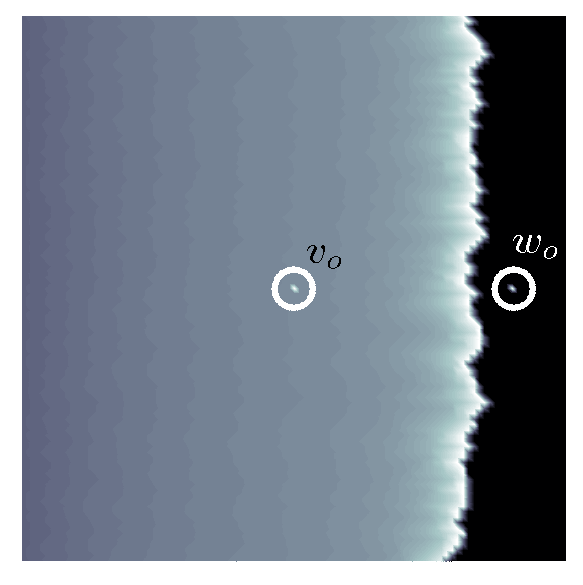
\epsfig{file = ./images/02_chap/Plano_Dinamica.eps,width = 4.5cm} &
 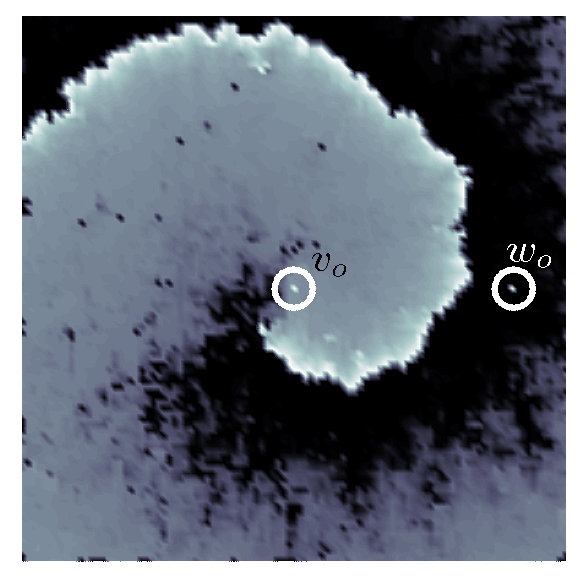
\epsfig{file = ./images/02_chap/Espiral_Dinamica.eps,width = 4.5cm} &
 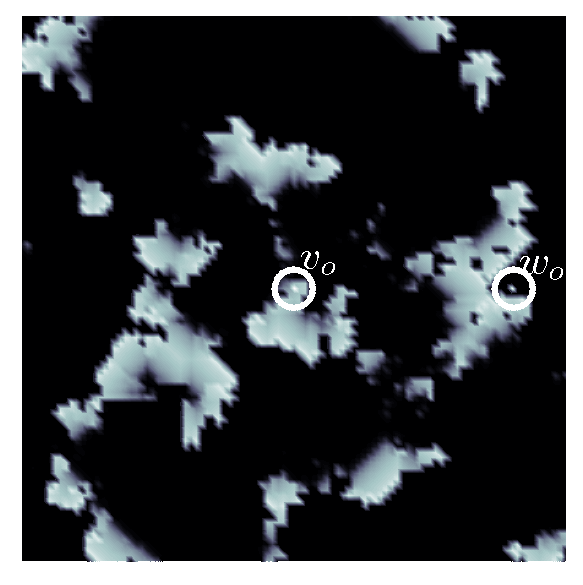
\epsfig{file = ./images/02_chap/Caos_Dinamica.eps,width = 4.5cm}\\
 (a)  & (b) &  (c)
 \end{tabular}
  \caption{ejemplo de dipolos (a) perfectamente correlacionados, (b))
  parcialmente correlacionados y (c) perfectamente incorrelacionadas .}
  \label{fig:din�micas}
\end{figure}

\subsection{Grado de auto-correlaci�n del tejido cardiaco}

El grado de auto-correlaci�n de una regi�n nos da el porcentaje de dipolos correlacionados dentro del volumen cardiaco. Se cuantifica la relaci�n entre los dipolos del tejido cardiaco, a trav�s del promediado del n�mero de dipolos correlacionados  en cada mapa de intensidades pico.

En este sentido, si la regi�n de auto-correlaci�n es homog�nea, podemos  hablar de �reas perfectamente  auto-correlacionadas cuando todos sus elementos est�n correlacionados entre si, y de �reas  perfectamente incorrelacionadas cuando todos los elementos de  la regi�n no satisfacen el  grado de correlaci�n, es decir su intensidad pico es nula.  Si la regi�n de auto-correlaci�n presenta diferentes intensidades de correlaci�n total, nosotros definimos umbrales de correlaci�n y de esta forma, se  clasifican las din�micas parcialmente correlacionadas.
 
En este orden y en funci�n de un umbral de correlaci�n, nosotros definimos la funci�n boleana para todos los elementos del mapa de intensidades pico de correlaci�n, como:
 
\begin{equation}
 \boldsymbol{U}(v,w)=
 \begin{cases}
    \begin{tabular}{ll}
        ${1}$ & if ${r}(v,w) > {u}$\\
        ${0}$ & otherwise
    \end{tabular}
 \end{cases}
\end{equation}

 La intensidad pico de correlaci�n total de los  dipolos  $\mathbf{J}(v_0,t)$ y $\mathbf{J}(w,t)$, esta definido por: 
\begin{equation}
{r}(v_o,w)  =max{|{R'_{J}}(v_o,w,\tau)|}
\end{equation}

Donde ${r}(v_o,w)$, puede tomar valores entre 0 y 1, De esta forma, el mapa de intensidades pico de correlaci�n del dipolo $\mathbf{J}(v_0,t)$, contiene  todo los elementos correspondientes  a  ${r}(v_o,w)$,  donde $w$ denota cada uno de los dipolos de $V$. Si ${r}(v_o,w)=0$, decimos que los dipolos  $\mathbf{J}(v_0,t)$ y $\mathbf{J}(w,t)$, est�n perfectamente  incorrelacionados, cuando  ${r}(v_o,w)=1$, decimos que los dipolos  $\mathbf{J}(v_0,t)$ y $\mathbf{J}(w,t)$ est�n perfectamente correlacionados. Cuando  $w = v_o$, ${r}(v_o,w)$ es la intensidad m�xima de la auto-correlaci�n del dipolo $\mathbf{J}(v_0,t)$, por lo que ${r}(v_o,w)={r}(v_o,v_o)=1$.




Donde $u$ es el umbral de correlaci�n  normalizado  por encima del cual  consideramos que la intensidad pico de correlaci�n total ${r}(v,w)$ es satisfactoria, $u$ varia entre 0 y 1. Si la regi�n de auto-correlaci�n es heterog�nea, es de suponer que a mayor valor del umbral de correlaci�n es menor el radio de la regi�n de auto-correlaci�n. De esta manera, el grado de auto-correlaci�n del tejido cardiaco  se puede define como el promedio de la cantidad de  dipolos  correlacionados  para cada $\mathbf{U}(v.w) \in V$. 

\begin{equation}
{T}=\frac{1}{V^2}\int_{VxV}{\mathbf{U}(v,w){dvdw}}
\end{equation}

En consecuencia, basados en el umbral de correlaci�n,  el volumen  cardiaco se
caracteriza de acuerdo al grado de auto-correlaci�n,  en donde, en funci�n del 
porcentaje de dipolos que satisfacen la auto-correlaci�n hablamos de  tejido 
correlacionado o incorrelacionado. Si el tama�o de  la regi�n de
auto-correlaci�n  es equiparado  con el tama�o del tejido observado por el Lead
Field,  podemos hablar que el tejido cardiaco se aproxima a una din�mica
perfectamente  correlacionada, por el contrario cuando  el  tama�o  de la regi�n
de auto-correlaci�n  es significativamente menor que el volumen del  tejido,
hablamos de din�micas incorrelacionadas.

\subsection{Spectrum of Cardic Signal}

La estimaci�n de la densidad espectral de potencia,   tanto para el  dipolo como
para las se�ales cardiacas,  se realiza con el m�todo de Welch.  La resoluci�n
de la estimaci�n espectral depende  del  n�mero de muestra del  e nventanado y
del solapamiento del mismo. El c�lculo del promedio de periodogramas,  para
observar la  envolvente espectral en las diferentes resoluciones  de Lead Field 
en cada una de las din�mica simuladas, se realiza con una ventana  Hamming de
512  muestras y un solapamiento del 50\%. Para ilustrar la  relaci�n entre los  
espectro de las se�ales cardiacas del frente de onda plano y su din�mica 
temporal,  nosotros empleamos ventanas Hamming de 2048 muestras para la
estimaci�n del  espectro de potencia  y observar los arm�nicos de la se�al.

Las se�ales cardiacas de las tres din�micas simuladas (frente de onda plano, 
espiral y caos), son sintetizadas en los 8 tama�os de lead Field definidos, 
$A_1$, $A_2$, $A_3$, $A_4$, $A_5$, $A_6$, $A_7$ y $A_8$,. el tiempo total  de 
simulaci�n es de 60 s. Para la estimaci�n del espectro  y  los mapas de
correlaci�n  se toma un intervalo de 20 s. La  tasa de muestreo de las se�ales  
sintetizadas es de 500 Hz.

El espectro de las se�ales cardiacas  en la din�mica perfectamente correlacionada, como se expone en \cite{RequenaSpectral1}, tiene asociado la funci�n de diferencia de tiempos de activaci�n ${\zeta}(v,w)$. Las diferencias de  tiempo son estimadas a partir de los instantes de  despolarizaci�n  de los  dipolo $\mathbf{J}(v,t)$ y $\mathbf{J}(w,t)$.  Cuando $v=w  { \zeta}(v,w)=0$. Para  las cuatro resoluciones espaciales de mayor tama�o de LeadField  se generan la funciones de distribuci�n $F_{A_1}(\zeta)$, $F_{A_2}(\zeta)$, $F_{A_3}(\zeta)$, $F_{A_4}(\zeta)$, respectivamente, y constituyen la descripci�n espacial de los dipolos perfectamente correlacionados.  De esta forma, el espectro  de las se�ales cardiacas en din�micas perfectamente correlacionas es expresado por:

\begin{equation}
S_{C_o}(\omega)=S_{A_o}(\omega) \cdot  S_{J}(\omega)
\end{equation}

Donde, $S_{A_o}(\omega)$, es la transformada de  Fourier de la funcion de distribuci�n de  tiempos  $F_{A_o}(\zeta)$ y $S_{J}(\omega)$, es el espectro de un  dipolo del  tejido card�aco. por lo que, el espectro del las  se�ales cardiacas en el frente de onda plano, depende de la resoluci�n espacial de cada leadField que nosotros definimos. En consecuencia, nosotos calculamos a partir de la funcion de distribuci�n de  tiempos, $S_{A_1}(\omega)$, $S_{A_2}(\omega)$, $S_{A_3}(\omega)$, $S_{A_4}(\omega)$.



\subsection{spectrum of cardiac sources}

 
 The spectrum of a cardiac source, $\boldsymbol{\sigma}(v,w,f)$, $\forall v,w\in
 V$, corresponds to the collection of the cross-spectra between all pairs of
 dipoles in $V$, and is defined as
 \begin{eqnarray}\label{eq:spectrum_source}
 &&\boldsymbol{\sigma}(v,w,f) =\mathcal{F}[\boldsymbol{\rho}(v,w,\tau)]
 \nonumber \\
 &&=\left( \begin{array}{ccc}
 {\sigma}_{xx}(v,w, f) & {\sigma}_{xy}(v,w, f) & {\sigma}_{xz}(v,w, f) \\
 {\sigma}_{yx}(v,w, f) & {\sigma}_{yy}(v,w, f) & {\sigma}_{yz}(v,w, f) \\
 {\sigma}_{zx}(v,w, f) & {\sigma}_{zy}(v,w, f) & {\sigma}_{zz}(v,w, f)
 \end{array} \right)
 \end{eqnarray}
 where the operator $\mathcal{F}[\cdot]$ is applied to
 $\boldsymbol{\rho}(v,w,\tau)$ on a component-by-component basis. For instance,
 ${\sigma}_{zy}(v,w, f)$ is $\mathcal{F}[{\rho}_{zy}(v,w,\tau)]$. 
 
 We also define the \emph{total cross-correlation} $R_{J}(v,w,\tau)$ between two
 cardiac dipoles $\mathbf{J}(v,t)$ and $\mathbf{J}(w,t)$ as the sum of the
 entries of $\boldsymbol{\rho}(v,w,\tau)$ and the \emph{total cross-spectrum}
 $S_{J}(v,w,f)$ as the Fourier Transform of $R_{J}(v,w,\tau)$. Mathematically,
 they can be expressed as
 
 \begin{eqnarray}
 S_{J}(v,w,f)  &=&  \mathbf{1}^{T} \boldsymbol{\sigma}(v,w, f)  \mathbf{1}.
\label{total_spectrum}
\end{eqnarray}

 Finally, we define the \emph{normalized} cross-correlation
$\boldsymbol{\hat{\rho}}(v,w,\tau)$ as the matrix of entries
\begin{equation}\label{eq:normalized_autocorrelation_source}
\hat{\rho}_{ab}(v,w,\tau) = \frac{{\rho}_{ab}(v,w,\tau)}{\sqrt{{\rho}_{aa}(v,v,0){\rho}_{bb}(w,w,0)}}
\end{equation}
 where $a,b\in \{x,y,z\}$, and the \emph{normalized} total cross-correlation
$\hat{R}_{J}(v,w,\tau)$ as
\begin{equation}\label{normalized_total_corr}
\hat{R}_{J}(v,w,\tau)= \frac{R_{J}(v,w,\tau)}{{\underset{\tau}{\max}}\{R_{J}(v,w,\tau)\}}.
\end{equation}




\section{M�todos estimaci�n del espectro}
\section{Frecuencia Dominante}

hablar aca de Fischer  \cite{Fischer07} y de Berenfeld \cite{Berenfeld10},
\cite{Berenfeld11} ,\cite{Berenfeld07}, \cite{Berenfeld10}

\section{Concluciones}

 

\part{An�lisis y Simulaciones} 

\chapter{Análisis}

\begin{resumen}

En este capitulo se realiza el análisis sistemático,  que conecta el espectro de las señales cardiacas con las características espacio temporal de diferentes dinámicas cardiacas, como, ritmos cardiacas altamente organizados, ritmos altamente desorganizados y ritmos parcialmente organizados. Las tres dinámicas de segundo orden,  se modelan  como \acf{FC}, \acf{FI} \acf{FPC}, respectivamente.

El capitulo inicia con la definición  del modelo espaciotemporal \acf{ID}, lo que permite relacionar los modelos de segundo orden con el espectro de las señales adquiridas en arritmias cardiacas. En este sentido se presenta la definición del  espectro de los modelos \ac{FC}, \ac{FI} \ac{FPC} y la respectiva autocorrelación.

A continuación. se presenta la definición y el análisis matemático  de \acf{MSD}, propuesta de  cuantificación de la resolución espacial del sistema de electrodo. Así mismo, se analizan las principales propiedades de la distribución de tiempos de activación, para darle una base sólida en función de la correlación de la  actividad cardiaca.
  

 \commentDir{ ... }

\end{resumen}

\section{Introducción}
\section{Modelos de fuentes de 2 orden}
\subsection{Dinámica Espacio-temporal de \acf{ID}}

% In this model of spatiotemporal dynamics all cardiac dipoles have the same autocorrelation and spectrum,
% \begin{eqnarray}
% \boldsymbol{\rho}(v,v,\tau)=\boldsymbol{\rho}(\tau), \label{corr_IDS}\\
% \boldsymbol{\sigma}(v,v,f)=\boldsymbol{\sigma}(f). \label{spectrum_IDS}
% \end{eqnarray}
% By substituting \eqref{corr_IDS} and \eqref{spectrum_IDS} respectively into \eqref{total_corr} and \eqref{total_spectrum}, it can be proved that the total autocorrelation and total spectrum of all the dipoles are also identical,
% \begin{eqnarray}
% R_{J}(v,v,\tau)&=&R_{J}(\tau)=\mathbf{1}^{T} \boldsymbol{\rho}(\tau)  \mathbf{1},\label{total_corr_IDS}\\
% S_{J}(v,v,f)&=&S_{J}(f)=\mathbf{1}^{T} \boldsymbol{\sigma}(f)  \mathbf{1}. \label{total_spectrum_IDS}
% \end{eqnarray}
% Note that this model only describes the activity of cardiac dipoles individually, and does not specify $\boldsymbol{\rho}(v,w,\tau)$ nor $\boldsymbol{\sigma}(v,w,f)$ for $v\neq w$.
%
\subsection{Dinámicas Espacio-temporales completamente correlacionadas }

% This model of spatiotemporal dynamics corresponds to highly regular rhythms, such as sinus rhythm, in which the activity of one dipole $\mathbf{J}(w,t)$ can be expressed as a delayed version of the activity of another dipole $\mathbf{J}(v,t)$,
% \begin{equation}\label{def:FCS}
% \mathbf{J}(w,t)=\mathbf{J}(v,t-\zeta (v,w)),
% \end{equation}
% where $\zeta (v,w)$ is defined as the time delay between the activities of dipoles $\mathbf{J}(v,t)$ and $\mathbf{J}(w,t)$. Based on \eqref{def:FCS}, it can be proved (see Appendix B) that FC dynamics are also ID, $\boldsymbol{\rho}(v,v,\tau)=\boldsymbol{\rho}(\tau)$ and $\boldsymbol{\sigma}(v,v,f)=\boldsymbol{\sigma}(f)$ [cf. \eqref{corr_IDS} and \eqref{spectrum_IDS}],  and that the autocorrelation and the spectrum of FC sources can be expressed as:
% \begin{eqnarray}
% \boldsymbol{\rho}(v,w,\tau) &=&\boldsymbol{\rho}(\tau - \zeta (v,w)), \label{eq:autocorrelation_correlated1}\\
% \boldsymbol{\sigma}(v,w,f) &=& \boldsymbol{\sigma}(f) \exp[-j2\pi f \zeta (v,w)]. \label{eq:spectrum_correlated}
% \end{eqnarray}
% Consequently, FC sources are completely characterized by $\boldsymbol{\rho}(\tau)$, $\boldsymbol{\sigma}(f)$ and $\zeta (v,w)$.
%

\subsection{Dinámicas Espacio-temporales completamente Incorrelacionadas}

% This model of spatiotemporal dynamics constitutes an idealization of highly irregular and disorganized rhythms, such as fibrillation, in which there is no second-order relationship between the temporal activity of any pair of cardiac dipoles. The autocorrelation and the spectrum of a FU source are defined as
% \begin{eqnarray}
% \boldsymbol{\rho}(v,w,\tau)=\boldsymbol{\rho}(v,v,\tau)\delta(v-w),\label{eq:autocorrelation_uncorrelated} \\
% \boldsymbol{\sigma}(v,w,\tau)=\boldsymbol{\sigma}(v,v,\tau)\delta(v-w).\label{eq:spectrum_uncorrelated}
% \end{eqnarray}
% In words, the cross-correlation between two cardiac dipoles $\mathbf{J}(w,t)$ and $\mathbf{J}(v,t)$, where $v\neq w$, is null.
%
%

\subsection{Dinámicas Espacio-temporales parcialmente correlacionadas}


\section{Función de distribución de tiempos}



\section{\acf{MSD}}

\subsection{Lead Fields}

\subsubsection{Modelo ideal}

% in this section we define one simple, idealized model of MSD, namely the pulse
% model. The pulse model describes a lead system that measures with the same
% sensitivity every dipole within a region $V_0$ of the volume source $V$, while
% rejecting the rest. Mathematically, this model is defined as
%
% \begin{equation}
% \label{def:pulso}
% \mathbf{L}_{V_0}(v)=
% \begin{cases}
%     \begin{tabular}{ll}
%     $\mathbf{1}$ & if $v\in V_0$\\
%     $\mathbf{0}$ & otherwise
%         \end{tabular}
%  \end{cases}.
% \end{equation}
%
% The pulse model can be treated as an approximation of physical MSD that
% effectively concentrate their measurement in a region $V_0$.
%
% For the subsequent analysis it is also convenient to quantify the spatial
% resolution (SR) of pulse leads. The SR can be defined as the region of the
% cardiac source that contributes the most to the measured signal. In this study
% we quantify the SR of pulse leads by introducing the notion of the lead
% equivalent volume (LEV), which is defined as the relative size of $V_{0}$ to
% the size of $V$,
%
% \begin{equation}
% LEV=\frac{\int_{V_{0}}{dv}}{\int_{V}{dv}}=\frac{M_{V_{0}}}{M_V},\label{eq:SR}
% \end{equation}
% where $M_{V_{0}}$ and $M_V$ are the sizes of $V_{0}$ and $V$ respectively.
% Thus, for local measurements the LEV is close to zero, whereas for global
% measurements where $V_0\simeq V$, the LEV is close to one.
%
%
\section{Resolución Espacial vs Ancho de Banda}

% we identify the relationship between: the spectrum of cardiac signals,
% the spatiotemporal dynamics of cardiac sources and the measurement
% characteristics of lead systems


\section{Concluciones}
\chapter{Simulaciones}
\begin{resumen}

Este capitulo utilizar el formalismo matemático presentado anteriormente, para analizar en un marco simulado la relación entre el volumen de correlación y el espectro captado por el sistema de electrodos.

Por medio de la implementación de diferentes modelos de la anatomía de tejido cardiaco, y junto a la simulación de diversos sistemas de electrodos, se simulan distintas dinámicas con distintas correlaciones  para ilustrar los resultados analíticos del capítulo anterior.

\commentDir{ ... }

\end{resumen}

\section{Introducción}
% el objetivo es generar dinámicas controladas, con respecto al nivel de
% correlación, ver mapas de correlación

\subsection{Tablas de experimentos}

\section{Implementación de modelos}
\subsection{Modelo de ruido blanco}
\subsection{Modelo Autómata}
\subsubsection{Protocolos de estimulacón}
\subsection{Modelo 2}
\subsection{Modelo 3}
\subsection{Modelo 4}

\section{Modelos de leadfield}

\section{Resolución espacial del sistemas de electrodos}
\section{Relación ancho de banda}


\section{Concluciones}



\part{Discusi�n y Conclusiones}
\chapter{Conclusiones}

acá esta



\newpage


%%-------------------FINAL DE LOS CAP�TULOS DE LA TESIS-------------%

% Ap�ndices
\part{Ap�ndices}
\appendix 
% -*-coding: iso-latin-1  -*-
sssss


% \nocite{*}

\backmatter % se usa para el estilo de la parte final del libro (la
% bibliograf�a, los ��ndices de materias).

% \bibliographystyle{IEEEtran}  
 \bibliographystyle{plainnat}
 \begin{small}
   \bibliography{biblio_tesis}
 \end{small}
\addcontentsline{toc}{chapter}{Bibliograf�a} 
 
\end{document}
